\section{\Arrays}
\label{arrays}

\RU{Массив это просто набор переменных в памяти, 
обязательно лежащих рядом и обязательно одного типа%
\footnote{\ac{AKA} \q{гомогенный контейнер}}.}
\EN{An array is just a set of variables in memory 
that lie next to each other and that have the same type%
\footnote{\ac{AKA} \q{homogeneous container}}.}
\DEph{}

% sections
\subsection{\RU{Простой пример}\EN{Simple example}}

\label{arrays_simple}
\lstinputlisting[style=customc]{patterns/13_arrays/1_simple/simple.c}

\EN{\subsubsection{x86}

\myparagraph{MSVC}

Let's compile:

\lstinputlisting[caption=MSVC 2008,style=customasmx86]{patterns/13_arrays/1_simple/simple_msvc.asm}

\myindex{x86!\Instructions!SHL}

Nothing very special, just two loops: the first is a filling loop and second is a printing loop.
The \TT{shl ecx, 1} instruction is used for value multiplication by 2 in \ECX, more about below~\myref{SHR}.

80 bytes are allocated on the stack for the array, 20 elements of 4 bytes.

\clearpage
Let's try this example in \olly.
\myindex{\olly}

We see how the array gets filled: 

each element is 32-bit word of \Tint type and its value is the index multiplied by 2:

\begin{figure}[H]
\centering
\myincludegraphics{patterns/13_arrays/1_simple/olly.png}
\caption{\olly: after array filling}
\label{fig:array_simple_olly}
\end{figure}

Since this array is located in the stack, we can see all its 20 elements there.

\myparagraph{GCC}

Here is what GCC 4.4.1 does:

\lstinputlisting[caption=GCC 4.4.1,style=customasmx86]{patterns/13_arrays/1_simple/simple_gcc.asm}

By the way, variable $a$ is of type  \IT{int*} 
(the pointer to \Tint{})---you can pass a pointer to an array to another function,
but it's more correct to say that a pointer to the first element of the array is passed
(the addresses of rest of the elements are calculated in an obvious way).

If you index this pointer as \IT{a[idx]}, \IT{idx} is just to be added to the pointer 
and the element placed there (to which calculated pointer is pointing) is to be returned.

An interesting example: a string of characters like 
\IT{\q{string}} is an array of characters and it has a type of \IT{const char[]}.

An index can also be applied to this pointer.

And that is why it is possible to write things like \TT{\q{string}[i]}---this is a correct \CCpp expression!

}
\RU{\subsubsection{x86}

\myparagraph{MSVC}

Компилируем:

\lstinputlisting[caption=MSVC 2008,style=customasmx86]{patterns/13_arrays/1_simple/simple_msvc.asm}

\myindex{x86!\Instructions!SHL}
Ничего особенного, просто два цикла. Один изменяет массив, второй печатает его содержимое. 
Команда \INS{shl ecx, 1} используется для умножения \ECX на 2, об этом ниже~(\myref{SHR}).

Под массив выделено в стеке 80 байт, это 20 элементов по 4 байта.

\clearpage
Попробуем этот пример в \olly.
\myindex{\olly}

Видно, как заполнился массив: каждый элемент это 32-битное слово типа \Tint, с шагом 2:

\begin{figure}[H]
\centering
\myincludegraphics{patterns/13_arrays/1_simple/olly.png}
\caption{\olly: после заполнения массива}
\label{fig:array_simple_olly}
\end{figure}

А так как этот массив находится в стеке, то мы видим все его 20 элементов внутри стека.

\myparagraph{GCC}

Рассмотрим результат работы GCC 4.4.1:

\lstinputlisting[caption=GCC 4.4.1,style=customasmx86]{patterns/13_arrays/1_simple/simple_gcc.asm}

Переменная $a$ в нашем примере имеет тип \IT{int*} (указатель на \Tint{}).
Вы можете попробовать передать в другую функцию указатель на массив,
но точнее было бы сказать, что передается указатель на первый элемент массива
(а адреса остальных элементов массива можно вычислить очевидным образом).

Если индексировать этот указатель как \IT{a[idx]}, \IT{idx} просто прибавляется к указателю 
и возвращается элемент, расположенный там, куда ссылается вычисленный указатель.

Вот любопытный пример. Строка символов вроде \IT{\q{string}} это массив из символов. 
Она имеет тип \IT{const char[]}.
К этому указателю также можно применять индекс.

Поэтому можно написать даже так:  \TT{\q{string}[i]}~--- это совершенно легальное выражение в \CCpp!

}
\DE{\subsubsection{x86}

\myparagraph{MSVC}

Kompilieren wir das Beispiel:

\lstinputlisting[caption=MSVC 2008,style=customasmx86]{patterns/13_arrays/1_simple/simple_msvc.asm}

\myindex{x86!\Instructions!SHL}
Soweit nichts Außergewöhnliches, nur zwei Schleifen: die erste füllt mit Werten auf und die zweite gibt Werte aus.
Der Befehl \TT{shl ecx, 1} wird für die Multiplikation mit 2 in \ECX verwendet; mehr dazu unten~\myref{SHR}.

Auf dem Stack werden 80 Bytes für das Array reserviert: 20 Elemente von je 4 Byte.

\clearpage
Untersuchen wir dieses Beispiel in \olly.
\myindex{\olly}

Wir erkennen wie das Array befüllt wird:

jedes Element ist ein 32-Bit-Wort vom Typ \Tint und der Wert ist der Index multipliziert mit 2:

\begin{figure}[H]
\centering
\myincludegraphics{patterns/13_arrays/1_simple/olly.png}
\caption{\olly: nach dem Füllen des Arrays}
\label{fig:array_simple_olly}
\end{figure}
Da sich dieses Array auf dem Stack befindet, finden wir dort alle seine 20 Elemente.

\myparagraph{GCC}

Hier ist was GCC 4.4.1 erzeugt:

\lstinputlisting[caption=GCC 4.4.1,style=customasmx86]{patterns/13_arrays/1_simple/simple_gcc.asm}
Die Variable $a$ ist übrigens vom Typ \IT{int*} (Pointer auf \Tint{})--man kann einen Pointer auf ein Array an eine
andere Funktion übergeben, aber es ist richtiger zu sagen, dass der Pointer auf das erste Element des Arrays übergeben
wird. (Die Adressen der übrigen Elemente werden in bekannter Weise berechnet.)

Wenn man diesen Pointer mittels \IT{a[idx]} indiziert, wird \IT{idx} zum Pointer addiert und das dort abgelegte Element
(auf das der berechnete Pointer zeigt) wird zurückgegeben.

Ein interessantes Beispiel: ein String wie \IT{\q{string}} ist ein Array von Chars und hat den Typ \IT{const
char[]}.

Auch auf diesen Pointer kann ein Index angewendet werden.

Das ist der Grund warum es es möglich ist, Dinge wie \TT{\q{string}[i]} zu schreiben--es handelt sich dabei um einen
korrekten \CCpp Ausdruck!

}

\EN{\subsubsection{ARM}

\myparagraph{\NonOptimizingKeilVI (\ARMMode)}

\lstinputlisting[style=customasmARM]{patterns/13_arrays/1_simple/simple_Keil_ARM_O0_EN.asm}

\Tint type requires 32 bits for storage (or 4 bytes),

so to store 20 \Tint variables 80 (\TT{0x50}) bytes are needed.
So that is why the \INS{SUB SP, SP, \#0x50} 

instruction in the function's prologue allocates exactly this amount of space in the stack.

In both the first and second loops, the loop iterator \var{i} is placed in the \Reg{4} register.

\myindex{ARM!Optional operators!LSL}

The number that is to be written into the array is calculated as $i*2$, which is effectively equivalent 
to shifting it left by one bit,\\
so \INS{MOV R0, R4,LSL\#1} instruction does this.

\myindex{ARM!\Instructions!STR}
\INS{STR R0, [SP,R4,LSL\#2]} writes the contents of \Reg{0} into the array.

Here is how a pointer to array element is calculated: \ac{SP} points to the start of the array, \Reg{4} is $i$.

So shifting $i$ left by 2 bits is effectively equivalent to multiplication by 4
(since each array element has a size of 4 bytes) and then it's added to the address of the start of the array.

\myindex{ARM!\Instructions!LDR}

The second loop has an inverse \INS{LDR R2, [SP,R4,LSL\#2]}
instruction. It loads the value we need from the array, and the pointer to it is calculated likewise.

\myparagraph{\OptimizingKeilVI (\ThumbMode)}

\lstinputlisting[style=customasmARM]{patterns/13_arrays/1_simple/simple_Keil_thumb_O3_EN.asm}

Thumb code is very similar.
\myindex{ARM!\Instructions!LSLS}

Thumb mode has special instructions for bit shifting (like \TT{LSLS}),
which calculates the value to be written into the array and the address of each element in the array as well.

The compiler allocates slightly more space in the local stack, however, the last 4 bytes are not used.

\myparagraph{\NonOptimizing GCC 4.9.1 (ARM64)}

\lstinputlisting[caption=\NonOptimizing GCC 4.9.1 (ARM64),style=customasmARM]{patterns/13_arrays/1_simple/ARM64_GCC491_O0_EN.s}

}
\RU{\subsubsection{ARM}

\myparagraph{\NonOptimizingKeilVI (\ARMMode)}

\lstinputlisting[style=customasmARM]{patterns/13_arrays/1_simple/simple_Keil_ARM_O0_RU.asm}

Тип \Tint требует 32 бита для хранения (или 4 байта),

так что для хранения 20 переменных типа \Tint, нужно 80 (\TT{0x50}) байт.

Поэтому инструкция \INS{SUB SP, SP, \#0x50} 
в прологе функции выделяет в локальном стеке под массив именно столько места.

И в первом и во втором цикле итератор цикла \var{i} будет постоянно находится в регистре \Reg{4}.

\myindex{ARM!Optional operators!LSL}
Число, которое нужно записать в массив, вычисляется так: $i*2$, и это эквивалентно 
сдвигу на 1 бит влево,\\
так что инструкция \INS{MOV R0, R4,LSL\#1} делает это.

\myindex{ARM!\Instructions!STR}
\INS{STR R0, [SP,R4,LSL\#2]} записывает содержимое \Reg{0} в массив.
Указатель на элемент массива вычисляется так: \ac{SP} указывает на начало массива, \Reg{4} это $i$.

Так что сдвигаем $i$ на 2 бита влево, что эквивалентно умножению на 4 
(ведь каждый элемент массива занимает 4 байта) и прибавляем это к адресу начала массива.

\myindex{ARM!\Instructions!LDR}
Во втором цикле используется обратная инструкция\\
\INS{LDR R2, [SP,R4,LSL\#2]}.
Она загружает из массива нужное значение и указатель на него вычисляется точно так же.

\myparagraph{\OptimizingKeilVI (\ThumbMode)}

\lstinputlisting[style=customasmARM]{patterns/13_arrays/1_simple/simple_Keil_thumb_O3_RU.asm}

Код для Thumb очень похожий.
\myindex{ARM!\Instructions!LSLS}
В Thumb имеются отдельные инструкции для битовых сдвигов (как \TT{LSLS}), 
вычисляющие и число для записи в массив и адрес каждого элемента массива.

Компилятор почему-то выделил в локальном стеке немного больше места, 
однако последние 4 байта не используются.

\myparagraph{\NonOptimizing GCC 4.9.1 (ARM64)}

\lstinputlisting[caption=\NonOptimizing GCC 4.9.1 (ARM64),style=customasmARM]{patterns/13_arrays/1_simple/ARM64_GCC491_O0_RU.s}

}
\DE{\subsubsection{ARM}

\myparagraph{\NonOptimizingKeilVI (\ARMMode)}

\lstinputlisting[style=customasmARM]{patterns/13_arrays/1_simple/simple_Keil_ARM_O0_DE.asm}

Der Typ \Tint benötigt 32 Bit (oder 4 Byte) zum Speichern, weshalb zum Speichern von 20 \Tint Variablen 80 (\TT{0x50})
Bytes benötigt werden. Deshalb reserviert der Befehl \INS{SUB SP, SP, \#0x50} im Funktionsprolog genau diese Menge an
Speicherplatz auf dem Stack.

In sowohl der ersten als auch der zweiten Scheife befindet sich der Scheifenzähler \var{i} im \Reg{4} Register.

\myindex{ARM!Optional operators!LSL}
Die Zahl, die in das Array geschrieben wird, wird über den Ausdruck $i\cdot 2$ berechnet, was äquivalent zur
Linksverschiebung um 1 Bit ist, weshalb der Befehl \INS{MOV R0, R4,LSL\#1} verwendet wird.

\myindex{ARM!\Instructions!STR}
\INS{STR R0, [SP,R4,LSL\#2]} schreibt den Inhalt von \Reg{0} in das Array.

Ein Pointer auf ein Arrayelement wird wie folgt berechnet: \ac{SP} zeigt auf den Beginn des Arrays, Reg{4} ist $i$.
Eine Linksverschiebung von $i$ um 2 Bits entspricht effektiv einer Multiplikation mit 4 (da jedes Arrayelement eine
Größe von 4 Byte hat) und wird dann zur Adresse am Beginn des Arrays addiert.

\myindex{ARM!\Instructions!LDR}
Die zweite Schleife enthält den inversen Befehl \INS{LDR R2, [SP,R4,LSL\#2]}. Er lädt den benötigten Wert aus dem Array
und der Pointer hierauf wird analog berechnet.

\myparagraph{\OptimizingKeilVI (\ThumbMode)}

\lstinputlisting[style=customasmARM]{patterns/13_arrays/1_simple/simple_Keil_thumb_O3_DE.asm}

Der Thumb Code ist sehr ähnlich.
\myindex{ARM!\Instructions!LSLS}
Der Thumb mode kennt spezielle Befehl für das bitweise Verschieben (wie \TT{LSLS}), der den in das Array zu schreibenden
Wert und die Adresse jedes Elements im Array berechnet.

Der Compiler reserviert ein wenig mehr Platz auf dem lokalen Stack, aber die letzten 4 Byte davon werden nicht
verwendet.

\myparagraph{\NonOptimizing GCC 4.9.1 (ARM64)}

\lstinputlisting[caption=\NonOptimizing GCC 4.9.1
(ARM64),style=customasmARM]{patterns/13_arrays/1_simple/ARM64_GCC491_O0_DE.s}

}

\EN{\subsubsection{MIPS}
% FIXME better start at non-optimizing version?

The function uses a lot of S- registers which must be preserved, so that's why its 
values are saved in the function prologue and restored in the epilogue.

\lstinputlisting[caption=\Optimizing GCC 4.4.5 (IDA),style=customasmMIPS]{patterns/13_arrays/1_simple/MIPS_O3_IDA_EN.lst}

Something interesting: there are two loops and the first one doesn't need $i$, it needs only 
$i*2$ (increased by 2 at each iteration) and also the address in memory (increased by 4 at each iteration).

So here we see two variables, one (in \$V0) increasing by 2 each time, and another (in \$V1) --- by 4.

The second loop is where \printf is called and it reports the value of $i$ to the user, 
so there is a variable
which is increased by 1 each time (in \$S0) and also a memory address (in \$S1) increased by 4 each time.

That reminds us of loop optimizations we considered earlier: \myref{loop_iterators}.

Their goal is to get rid of of multiplications.

}
\RU{\subsubsection{MIPS}
% FIXME better start at non-optimizing version?
Функция использует много S-регистров, которые должны быть сохранены. Вот почему их значения сохраняются
в прологе функции и восстанавливаются в эпилоге.

\lstinputlisting[caption=\Optimizing GCC 4.4.5 (IDA),style=customasmMIPS]{patterns/13_arrays/1_simple/MIPS_O3_IDA_RU.lst}

Интересная вещь: здесь два цикла и в первом не нужна переменная $i$, а нужна только переменная
$i*2$ (скачущая через 2 на каждой итерации) и ещё адрес в памяти (скачущий через 4 на каждой итерации).

Так что мы видим здесь две переменных: одна (в \$V0) увеличивается на 2 каждый раз, и вторая (в \$V1) --- на 4.

Второй цикл содержит вызов \printf. Он должен показывать значение $i$ пользователю,
поэтому здесь есть переменная, увеличивающаяся на 1 каждый раз (в \$S0), а также адрес в памяти (в \$S1) 
увеличивающийся на 4 каждый раз.

Это напоминает нам оптимизацию циклов, которую мы рассматривали ранее: \myref{loop_iterators}.
Цель оптимизации в том, чтобы избавиться от операций умножения.

}
\DE{\subsubsection{MIPS}
% FIXME better start at non-optimizing version?
Die Funktion verwendet eine Menge S-Register, die gesichert werden müssen. Das ist der Grund dafür, dass die Werte im
Funktionsprolog gespeichert und im Funktionsepilog wiederhergestellt werden.

\lstinputlisting[caption=\Optimizing GCC 4.4.5
(IDA),style=customasmMIPS]{patterns/13_arrays/1_simple/MIPS_O3_IDA_DE.lst}
Interessant: es gibt zwei Schleifen und die erste benötigt $i$ nicht; sie benötigt nur $i\cdot 2$ (erhöht um 2 bei
jedem Iterationsschritt) und die Adresse im Speicher (erhöht um 4 bei jedem Iterationsschritt).

Wir sehen hier also zwei Variablen: eine (in \$V0), die jedes Mal um 2 erhöht wird, und eine andere (in\$V1), die um 4
erhöht wird.

Die zweite Schleife ist der Ort, an dem \printf aufgerufen wird und dem Benutzer den Wert von $i$ zurückliefert, es gibt
also eine Variable die in \$S0 inkrementiert wird und eine Speicheradresse in \$S1, die jedes Mal um 4 erhöht wird.

Das erinnert uns an die Optimierung von Schleifen, die wir früher betrachtet haben: \myref{loop_iterators}.

Das Ziel der Optimierung ist es, die Multiplikationen loszuwerden.}


\subsection{\RU{Переполнение буфера}\EN{Buffer overflow}}
\label{subsec:bufferoverflow}
\myindex{\BufferOverflow}

\EN{\subsubsection{Reading outside array bounds}

So, array indexing is just \IT{array\lbrack{}index\rbrack}.
If you study the generated code closely, you'll probably note the missing index bounds checking,
which could check \IT{if it is less than 20}.
What if the index is 20 or greater?
That's the one \CCpp feature it is often blamed for.

Here is a code that successfully compiles and works:

\lstinputlisting[style=customc]{patterns/13_arrays/2_BO/r.c}

Compilation results (MSVC 2008):

\lstinputlisting[caption=\NonOptimizing MSVC 2008,style=customasmx86]{patterns/13_arrays/2_BO/r_msvc.asm}

The code produced this result:

\lstinputlisting[caption=\olly: console output]{patterns/13_arrays/2_BO/console.txt}

It is just \IT{something} that has been lying in the stack near to the array, 80 bytes away from its first element.

\clearpage
\myindex{\olly}
Let's try to find out where did this value come from, using \olly.

Let's load and find the value located right after the last array element:

\begin{figure}[H]
\centering
\myincludegraphics{patterns/13_arrays/2_BO/olly_r1.png}
\caption{\olly: reading of the 20th element and execution of \printf}
\label{fig:array_BO_olly_r1}
\end{figure}

What is this? 
Judging by the stack layout,
this is the saved value of the EBP register.
\clearpage
Let's trace further and see how it gets restored:

\begin{figure}[H]
\centering
\myincludegraphics{patterns/13_arrays/2_BO/olly_r2.png}
\caption{\olly: restoring value of EBP}
\label{fig:array_BO_olly_r2}
\end{figure}

Indeed, how it could be different?
The compiler may generate some additional code to check the index value to be always
in the array's bounds (like in higher-level programming languages\footnote{Java, Python, etc.})
but this makes the code slower.

}
\RU{\subsubsection{Чтение за пределами массива}

Итак, индексация массива --- это просто \IT{массив\lbrack{}индекс\rbrack}.  % TODO1 как-то плохо отображаются []
Если вы присмотритесь к коду, в цикле печати значений массива через \printf вы 
не увидите проверок индекса, \IT{меньше ли он двадцати?} 
А что будет если он будет 20 или больше? 
Эта одна из особенностей \CCpp, за которую их, собственно, и ругают.

Вот код, который и компилируется и работает:

\lstinputlisting[style=customc]{patterns/13_arrays/2_BO/r.c}

Вот результат компиляции в (MSVC 2008):

\lstinputlisting[caption=\NonOptimizing MSVC 2008,style=customasmx86]{patterns/13_arrays/2_BO/r_msvc.asm}

Данный код при запуске выдал вот такой результат:

\lstinputlisting[caption=\olly: вывод в консоль]{patterns/13_arrays/2_BO/console.txt}

Это просто \IT{что-то}, что волею случая лежало в стеке рядом с массивом, 
через 80 байт от его первого элемента.

\clearpage
\myindex{\olly}
Попробуем узнать в \olly, что это за значение.
Загружаем и находим это значение, находящееся точно после последнего элемента массива:

\begin{figure}[H]
\centering
\myincludegraphics{patterns/13_arrays/2_BO/olly_r1.png}
\caption{\olly: чтение 20-го элемента и вызов \printf}
\label{fig:array_BO_olly_r1}
\end{figure}

Что это за значение? 
Судя по разметке стека, это сохраненное значение регистра EBP.
\clearpage
Трассируем далее, и видим, как оно восстанавливается:

\begin{figure}[H]
\centering
\myincludegraphics{patterns/13_arrays/2_BO/olly_r2.png}
\caption{\olly: восстановление EBP}
\label{fig:array_BO_olly_r2}
\end{figure}

Действительно, а как могло бы быть иначе? Компилятор мог бы встроить какой-то код, 
каждый раз проверяющий индекс на соответствие пределам массива, как в языках программирования 
более высокого уровня\footnote{Java, Python, итд.}, что делало бы запускаемый код медленнее.

}
\DE{\subsubsection{Lesezugriff außerhalb von Arraygrenzen}
Der indizierte Zugriff auf ein Array wird durch \IT{array\lbrack{}index\rbrack} realisiert.
Wenn man sich den erzeugten Code genau ansieht, bemerkt man, dass eine Prüfung der Indexgrenzen fehlt, welche die
Bedingung \IT{kleiner als 20} validiert.
Was also passiert, wenn der Index 20 oder größer ist? 
Hier haben wir es mit einem unschönen Feature von \CCpp zu tun

Hier ein Beipsielcode der erfolgreich kompiliert wurde und funktioniert:

\lstinputlisting[style=customc]{patterns/13_arrays/2_BO/r.c}

Ergebnis des Kompiliervorgangs (MSVC 2008):

\lstinputlisting[caption=\NonOptimizing MSVC 2008,style=customasmx86]{patterns/13_arrays/2_BO/r_msvc.asm}

Der Code produziert dieses Ergebnis:

\lstinputlisting[caption=\olly: console output]{patterns/13_arrays/2_BO/console.txt}
Es handelt sich um \IT{irgendetwas}, das auf dem Stack in der Nähe des Arrays gelegen hat, 80 Byte von dessen erstem
Element entfernt.

\clearpage
\myindex{\olly}
Versuchen wir mit \olly herauszufinden, woher dieser Wert kommt.

Laden und finden wir also den Wert, der sich direkt hinter dem letzten Arrayelement befindet:

\begin{figure}[H]
\centering
\myincludegraphics{patterns/13_arrays/2_BO/olly_r1.png}
\caption{\olly: das 20. Element lesen und \printf ausführen}
\label{fig:array_BO_olly_r1}
\end{figure}

Worum handelt es sich? 
Dem Stacklayout nach zu urteilen ist dies der gespeicherte Wert des EBP Registers.
\clearpage
Verfolgen wir das ganze weiter und schauen uns an, wie dieser wiederhergestellt wird:

\begin{figure}[H]
\centering
\myincludegraphics{patterns/13_arrays/2_BO/olly_r2.png}
\caption{\olly: Wert von EBP wiederherstellen}
\label{fig:array_BO_olly_r2}
\end{figure}
Wie könnte es anders gelöst werden?
Der Compiler könnte zusätzlichen Code erzeugen, der sicherstellt, dass der Index sich stets innerhalb der Arraygrenzen
befindet (wie in höheren Programmiersprachen\footnote{Java, Python, etc.}), aber das würde den Code langsamer machen.
}

\EN{\subsubsection{Writing beyond array bounds}

OK, we read some values from the stack \IT{illegally}, but what if we could write something to it?

Here is what we have got:

\lstinputlisting[style=customc]{patterns/13_arrays/2_BO/w.c}

\myparagraph{MSVC}

And what we get:

\lstinputlisting[caption=\NonOptimizing MSVC 2008,style=customasmx86]{patterns/13_arrays/2_BO/w_EN.asm}

The compiled program crashes after running. No wonder. Let's see where exactly does it is crash.

\clearpage
\myindex{\olly}

Let's load it into \olly, and trace until all 30 elements are written:

\begin{figure}[H]
\centering
\myincludegraphics{patterns/13_arrays/2_BO/olly_w1.png}
\caption{\olly: after restoring the value of EBP}
\label{fig:array_BO_olly_w1}
\end{figure}

\clearpage
Trace until the function end:

\begin{figure}[H]
\centering
\myincludegraphics{patterns/13_arrays/2_BO/olly_w2.png}
\caption{\olly: 
\TT{EIP} has been restored, but \olly can't disassemble at 0x15}
\label{fig:array_BO_olly_w2}
\end{figure}

Now please keep your eyes on the registers.

\EIP is 0x15 now. It is not a legal address for code---at least for win32 code!
We got there somehow against our will.
It is also interesting that the \EBP register contain 0x14,
\ECX and \EDX contain 0x1D.

Let's study stack layout a bit more.

After the control flow has been passed to \TT{\main}, the value in the \EBP register was saved on the stack.
Then, 84 bytes were allocated for the array and the $i$ variable.
That's \TT{(20+1)*sizeof(int)}.
\ESP now points to the \TT{\_i} variable in the local stack and after the execution of 
the next \TT{PUSH something}, \IT{something} is appearing next to \TT{\_i}.

That's the stack layout while the control is in \main:

\begin{center}
\begin{tabular}{ | l | l | }
\hline
  \TT{ESP}    & 4 bytes allocated for $i$ variable \\
\hline
  \TT{ESP+4}  & 80 bytes allocated for \TT{a[20]} array \\
\hline
  \TT{ESP+84} & saved \EBP value \\
\hline
  \TT{ESP+88} & return address \\
\hline
\end{tabular}
\end{center}

\TT{a[19]=something} statement writes the last \Tint in the bounds of the array (in bounds so far!).

\TT{a[20]=something} statement writes \IT{something} to the place where the value of \EBP is saved.

Please take a look at the register state at the moment of the crash. In our case,
20 has been written in the 20th element. 
At the function end, the function epilogue restores the original \EBP value.
(20 in decimal is \TT{0x14} in hexadecimal).
Then \RET gets executed, which is effectively equivalent to \TT{POP EIP} instruction.

The \RET instruction takes the return address from the stack (that is the address in \ac{CRT}),
which has called \main),
and 21 is stored there (\TT{0x15} in hexadecimal).
The CPU traps at address \TT{0x15},
but there is no executable code there, so exception gets raised.

\myindex{\BufferOverflow}

Welcome! It is called a \IT{buffer overflow}\footnote{\href{http://go.yurichev.com/17132}{wikipedia}}.

Replace the \Tint array with a string (\Tchar array), create a long string deliberately
and pass it to the program, to the function, which doesn't check the length of the string and copies it in a short buffer,
and you'll able to point the program to an address to which it must jump.
It's not that simple in reality, but that is how it emerged.
Classic article about it: \AlephOne.

\myparagraph{GCC}

Let's try the same code in GCC 4.4.1. We get:

\lstinputlisting[style=customasmx86]{patterns/13_arrays/2_BO/w_gcc.asm}

Running this in Linux will produce: \TT{Segmentation fault}.

\myindex{GDB}

If we run this in the GDB debugger, we get this:

\begin{lstlisting}
(gdb) r
Starting program: /home/dennis/RE/1 

Program received signal SIGSEGV, Segmentation fault.
0x00000016 in ?? ()
(gdb) info registers
eax            0x0	0
ecx            0xd2f96388	-755407992
edx            0x1d	29
ebx            0x26eff4	2551796
esp            0xbffff4b0	0xbffff4b0
ebp            0x15	0x15
esi            0x0	0
edi            0x0	0
eip            0x16	0x16
eflags         0x10202	[ IF RF ]
cs             0x73	115
ss             0x7b	123
ds             0x7b	123
es             0x7b	123
fs             0x0	0
gs             0x33	51
(gdb) 
\end{lstlisting}

The register values are slightly different than in win32 example, 
since the stack layout is slightly different too.

}
\RU{\subsubsection{Запись за пределы массива}

Итак, мы прочитали какое-то число из стека явно \IT{нелегально}, а что если мы запишем?

Вот что мы пишем:

\lstinputlisting[style=customc]{patterns/13_arrays/2_BO/w.c}

\myparagraph{MSVC}

И вот что имеем на ассемблере:

\lstinputlisting[caption=\NonOptimizing MSVC 2008,style=customasmx86]{patterns/13_arrays/2_BO/w_RU.asm}

Запускаете скомпилированную программу, и она падает. Немудрено. Но давайте теперь узнаем, где именно.

\clearpage
\myindex{\olly}

Загружаем в \olly, трассируем пока запишутся все 30 элементов:

\begin{figure}[H]
\centering
\myincludegraphics{patterns/13_arrays/2_BO/olly_w1.png}
\caption{\olly: после восстановления EBP}
\label{fig:array_BO_olly_w1}
\end{figure}

\clearpage
Доходим до конца функции:

\begin{figure}[H]
\centering
\myincludegraphics{patterns/13_arrays/2_BO/olly_w2.png}
\caption{\olly: EIP восстановлен, но \olly не может дизассемблировать по адресу 0x15}
\label{fig:array_BO_olly_w2}
\end{figure}

Итак, следите внимательно за регистрами.

\EIP теперь 0x15. Это явно нелегальный адрес для кода~--- по крайней мере, win32-кода! 
Мы там как-то очутились, причем, сами того не хотели. Интересен также тот факт, что в \EBP хранится 0x14, 
а в \ECX и \EDX хранится 0x1D.

Ещё немного изучим разметку стека.

После того как управление передалось в \main, в стек было сохранено значение \EBP. 
Затем для массива и переменной $i$ было выделено 84 байта. Это \TT{(20+1)*sizeof(int)}. 
\ESP сейчас указывает на переменную \TT{\_i} в локальном стеке и при исполнении следующего \INS{PUSH что-либо}, 
\IT{что-либо} появится рядом с \TT{\_i}.

Вот так выглядит разметка стека пока управление находится внутри \main:

\begin{center}
\begin{tabular}{ | l | l | }
\hline
  \TT{ESP}    & 4 байта выделенных для переменной $i$ \\
\hline
  \TT{ESP+4}  & 80 байт выделенных для массива \TT{a[20]} \\
\hline
  \TT{ESP+84} & сохраненное значение \EBP \\
\hline
  \TT{ESP+88} & адрес возврата \\
\hline
\end{tabular}
\end{center}

Выражение \TT{a[19]=что\_нибудь} записывает последний \Tint в пределах массива (пока что в пределах!).

Выражение \TT{a[20]=что\_нибудь} записывает \IT{что\_нибудь} на место где сохранено значение \EBP.

Обратите внимание на состояние регистров на момент падения процесса. В нашем случае 
в 20-й элемент записалось значение 20. 
И вот всё дело в том, что заканчиваясь, эпилог функции восстанавливал значение \EBP 
(20 в десятичной системе это как раз \TT{0x14} в шестнадцатеричной). 
Далее выполнилась инструкция \RET, которая на самом деле эквивалентна \TT{POP EIP}.

Инструкция \RET вытащила из стека адрес возврата (это адрес где-то внутри \ac{CRT}), которая вызвала \main),
а там было записано 21 в десятичной системе, то есть 0x15 в шестнадцатеричной. 
И вот процессор оказался по адресу 0x15, но исполняемого кода там нет, так что случилось исключение.

\myindex{\BufferOverflow}
Добро пожаловать! Это называется \IT{buffer overflow}\footnote{\href{http://go.yurichev.com/17132}{wikipedia}}.

Замените массив \Tint на строку (массив \Tchar), нарочно создайте слишком длинную строку, 
передайте её в ту программу, 
в ту функцию, которая не проверяя длину строки скопирует её в слишком короткий буфер, 
и вы сможете указать программе, по какому именно адресу перейти. 
Не всё так просто в реальности, конечно, но началось всё с этого.
Классическая статья об этом: \AlephOne.

\myparagraph{GCC}

Попробуем то же самое в GCC 4.4.1. У нас выходит такое:

\lstinputlisting[style=customasmx86]{patterns/13_arrays/2_BO/w_gcc.asm}

Запуск этого в Linux выдаст: \TT{Segmentation fault}.

\myindex{GDB}
Если запустить полученное в отладчике GDB, получим:

\begin{lstlisting}
(gdb) r
Starting program: /home/dennis/RE/1 

Program received signal SIGSEGV, Segmentation fault.
0x00000016 in ?? ()
(gdb) info registers
eax            0x0	0
ecx            0xd2f96388	-755407992
edx            0x1d	29
ebx            0x26eff4	2551796
esp            0xbffff4b0	0xbffff4b0
ebp            0x15	0x15
esi            0x0	0
edi            0x0	0
eip            0x16	0x16
eflags         0x10202	[ IF RF ]
cs             0x73	115
ss             0x7b	123
ds             0x7b	123
es             0x7b	123
fs             0x0	0
gs             0x33	51
(gdb) 
\end{lstlisting}

Значения регистров немного другие, чем в примере win32, потому что разметка стека чуть другая.

}
\DE{\subsubsection{Schreibzugriff außerhalb von Arraygrenzen}
Nehmen wir an, wir hätte ein paar Werte illegalerweise vom Stack gelesen, wie könnten wir etwas hineinschreiben?

Hier ist, was wir haben:

\lstinputlisting[style=customc]{patterns/13_arrays/2_BO/w.c}

\myparagraph{MSVC}

Wir erhalten das Folgende:

\lstinputlisting[caption=\NonOptimizing MSVC 2008,style=customasmx86]{patterns/13_arrays/2_BO/w_DE.asm}
Das kompilierte Programm stürzt nach der Ausführung ab. Das verwundert nicht. Schauen wir, was genau den Absturz
verursacht.

\clearpage
\myindex{\olly}
Laden wir das Programm in \olly und verfolgen den Ablauf, bis alle 30 Elemente geschrieben worden sind:

\begin{figure}[H]
\centering
\myincludegraphics{patterns/13_arrays/2_BO/olly_w1.png}
\caption{\olly: nach Wiederherstellung des Wertes von EBP}
\label{fig:array_BO_olly_w1}
\end{figure}

\clearpage
Nachverfolgen bis zum Ende der Funktion:

\begin{figure}[H]
\centering
\myincludegraphics{patterns/13_arrays/2_BO/olly_w2.png}
\caption{\olly: 
\TT{EIP} wurde wiederhergestellt, aber \olly kann an 0x15 nicht disassemblieren}
\label{fig:array_BO_olly_w2}
\end{figure}
Richten wir unser Augenmerk auf die Register.

\EIP ist jetzt gerade 0x15. Das ist keine gültige Adreses für Code---zumindest nicht für win32 Code!
Interessant ist auch, dass das \EBP Register 0x14 enthält und \ECX sowie \EDX jeweils 0x1D

Schauen wir uns das Stacklayout etwas genauer an.

Nachdem der Control Flow an \TT{\main} übergeben worde ist, wurde der Wert in \EBP auf dem Stack abgelegt.
Danach wurden 84 Byte für das Array und die Variable $i$ reserviert.
Das entspricht \TT{(20+1)*sizeof(int)}.
\ESP zeigt jetzt auf die Variable \TT{\_i} im lokalen Stack und nach der Ausführung von \TT{PUSH something} scheint sich
\TT{something} neben \TT{\_i} zu befinden.

Hier ist das Stacklayout während der Control Flow in der \main ist:

\begin{center}
\begin{tabular}{ | l | l | }
\hline
  \TT{ESP}    & 4 Byte reserviert für Variable $i$ \\
\hline
  \TT{ESP+4}  & 80 Byte reserviert für Array \TT{a[20]} \\
\hline
  \TT{ESP+84} & sichere Wert von \EBP \\
\hline
  \TT{ESP+88} & Rücksprungadresse \\
\hline
\end{tabular}
\end{center}
Der Befehl \TT{a[19]=something} schreibt den letzten \Tint innerhalb der Grenzen des Arrays (bis hierhin ist alles in
Ordnung!).
Der Befehl \TT{a[20]=something} schreibt \IT{something} an die Stelle, an der der \EBP gespeichert ist.

Sehen wir uns den Zustand der Register im Moment des Absturzes an. In unserem Fall wurde 20 in das zwanzigste Element
geschrieben. Am Ende der Funktion stellt der Funktionsepilog den originalen Wert von \EBP wieder her.
(20 dezimal entspricht \TT{0x14} hexadezimal).
Danach wird \RET ausgeführt, was äquivalent zum Befehl \TT{POP EIP} ist.

Der Befehl \RET nimmt die Rücksprungadresse vom Stack (das ist die Adresse in \ac{CRT}, die \main aufgerufen hat) und
speichert hier den Wert 21 (\TT{0x15} hexadezimal).
Die CPU springt an die Adresse \TT{0x15}, aber hier befindet sich kein ausführbarer Code, sodass eine Exception geworfen
wird.

\myindex{\BufferOverflow}
Dies nennt man einen \IT{Buffer Overflow}\footnote{\href{http://go.yurichev.com/17132}{wikipedia}}.

Ersetzt man das \Tint Array durch einen String (\Tchar Array) und erzeugt absichtlich einen langen String und übergibt
ihn im Programm an eine Funktion, die die Länge des Strings nicht prüft und ihn in einen kurzen Buffer kopiert, kann man
das Programm zwingen an eine bestimmte Adresse zu springen.
In der Realität ist dieses Verhalten nicht so einfach zu erzeugen, funktioniert aber von Prinzip her genau wie hier.
Ein klassischer Artikel dazu:\AlephOne.

\myparagraph{GCC}

Kompilieren wir denselben Code mit GCC 4.4.1, erhalten wir:

\lstinputlisting[style=customasmx86]{patterns/13_arrays/2_BO/w_gcc.asm}

Lässt man das Programm unter Linux laufen, lautet das Ergebnis: \TT{Segmentation fault}.

\myindex{GDB}
Wenn wir es mit dem GDB Debugger laufen lassen, erhalten wir das Folgende:


\begin{lstlisting}
(gdb) r
Starting program: /home/dennis/RE/1 

Program received signal SIGSEGV, Segmentation fault.
0x00000016 in ?? ()
(gdb) info registers
eax            0x0	0
ecx            0xd2f96388	-755407992
edx            0x1d	29
ebx            0x26eff4	2551796
esp            0xbffff4b0	0xbffff4b0
ebp            0x15	0x15
esi            0x0	0
edi            0x0	0
eip            0x16	0x16
eflags         0x10202	[ IF RF ]
cs             0x73	115
ss             0x7b	123
ds             0x7b	123
es             0x7b	123
fs             0x0	0
gs             0x33	51
(gdb) 
\end{lstlisting}
Die Registerwerte unterscheiden sich geringfügig vom win32 Beispiel, da auch das Stacklayout ein wenig anders ist.
}


\EN{\subsection{Buffer overflow protection methods}
\label{subsec:BO_protection}

There are several methods to protect against this scourge, regardless of the \CCpp programmers' negligence.
MSVC has options like\footnote{compiler-side buffer overflow protection methods:
\href{http://go.yurichev.com/17133}{wikipedia.org/wiki/Buffer\_overflow\_protection}}:

\begin{lstlisting}
 /RTCs Stack Frame runtime checking
 /GZ Enable stack checks (/RTCs)
\end{lstlisting}

\myindex{x86!\Instructions!RET}
\myindex{Function prologue}
\myindex{Security cookie}

One of the methods is to write a random value between the local variables in stack at function prologue 
and to check it in function epilogue before the function exits.
If value is not the same, do not execute the last instruction \RET, but stop (or hang).
The process will halt, but that is much better than a remote attack to your host.
    
\newcommand{\CANARYURL}{\href{http://go.yurichev.com/17134}{wikipedia.org/wiki/Domestic\_canary\#Miner.27s\_canary}}

\myindex{Canary}

This random value is called a \q{canary} sometimes, it is related to the miners' canary\footnote{\CANARYURL},
they were used by miners in the past days in order to detect poisonous gases quickly.

Canaries are very sensitive to mine gases, they become very agitated in case of danger, or even die.

If we compile our very simple array example~(\myref{arrays_simple}) in \ac{MSVC}
with RTC1 and RTCs option,\\
you can see a call to \TT{@\_RTC\_CheckStackVars@8} a function at the end of the function that checks if the \q{canary} is correct.

Let's see how GCC handles this. 
Let's take an \TT{alloca()}~(\myref{alloca}) example:

\lstinputlisting[style=customc]{patterns/02_stack/04_alloca/2_1.c}

By default, without any additional options, GCC 4.7.3 inserts a \q{canary} check into the code:

\lstinputlisting[caption=GCC 4.7.3,style=customasmx86]{patterns/13_arrays/3_BO_protection/gcc_canary_EN.asm}

\myindex{x86!\Registers!GS}
The random value is located in \TT{gs:20}. 
It gets written on the stack and then at the end of the function
the value in the stack is compared with the correct \q{canary} in \TT{gs:20}. 
If the values are not equal, the 
\TT{\_\_stack\_chk\_fail} 
function is called and we can see in the console something like that (Ubuntu 13.04 x86):

\begin{lstlisting}
*** buffer overflow detected ***: ./2_1 terminated
======= Backtrace: =========
/lib/i386-linux-gnu/libc.so.6(__fortify_fail+0x63)[0xb7699bc3]
/lib/i386-linux-gnu/libc.so.6(+0x10593a)[0xb769893a]
/lib/i386-linux-gnu/libc.so.6(+0x105008)[0xb7698008]
/lib/i386-linux-gnu/libc.so.6(_IO_default_xsputn+0x8c)[0xb7606e5c]
/lib/i386-linux-gnu/libc.so.6(_IO_vfprintf+0x165)[0xb75d7a45]
/lib/i386-linux-gnu/libc.so.6(__vsprintf_chk+0xc9)[0xb76980d9]
/lib/i386-linux-gnu/libc.so.6(__sprintf_chk+0x2f)[0xb7697fef]
./2_1[0x8048404]
/lib/i386-linux-gnu/libc.so.6(__libc_start_main+0xf5)[0xb75ac935]
======= Memory map: ========
08048000-08049000 r-xp 00000000 08:01 2097586    /home/dennis/2_1
08049000-0804a000 r--p 00000000 08:01 2097586    /home/dennis/2_1
0804a000-0804b000 rw-p 00001000 08:01 2097586    /home/dennis/2_1
094d1000-094f2000 rw-p 00000000 00:00 0          [heap]
b7560000-b757b000 r-xp 00000000 08:01 1048602    /lib/i386-linux-gnu/libgcc_s.so.1
b757b000-b757c000 r--p 0001a000 08:01 1048602    /lib/i386-linux-gnu/libgcc_s.so.1
b757c000-b757d000 rw-p 0001b000 08:01 1048602    /lib/i386-linux-gnu/libgcc_s.so.1
b7592000-b7593000 rw-p 00000000 00:00 0
b7593000-b7740000 r-xp 00000000 08:01 1050781    /lib/i386-linux-gnu/libc-2.17.so
b7740000-b7742000 r--p 001ad000 08:01 1050781    /lib/i386-linux-gnu/libc-2.17.so
b7742000-b7743000 rw-p 001af000 08:01 1050781    /lib/i386-linux-gnu/libc-2.17.so
b7743000-b7746000 rw-p 00000000 00:00 0
b775a000-b775d000 rw-p 00000000 00:00 0
b775d000-b775e000 r-xp 00000000 00:00 0          [vdso]
b775e000-b777e000 r-xp 00000000 08:01 1050794    /lib/i386-linux-gnu/ld-2.17.so
b777e000-b777f000 r--p 0001f000 08:01 1050794    /lib/i386-linux-gnu/ld-2.17.so
b777f000-b7780000 rw-p 00020000 08:01 1050794    /lib/i386-linux-gnu/ld-2.17.so
bff35000-bff56000 rw-p 00000000 00:00 0          [stack]
Aborted (core dumped)
\end{lstlisting}

\myindex{MS-DOS}
gs is the so-called segment register. These registers were used widely in MS-DOS and DOS-extenders
times.
Today, its function is different.
\myindex{TLS}
\myindex{Windows!TIB}

To say it briefly, the \TT{gs} register in Linux always points to the
\ac{TLS}~(\myref{TLS})---some information specific to thread is stored there.
By the way, in win32 the \TT{fs} register plays the same role, pointing to
\ac{TIB} \footnote{\href{http://go.yurichev.com/17104}{wikipedia.org/wiki/Win32\_Thread\_Information\_Block}}. 

More information can be found in the Linux kernel source code (at least in 3.11 version),\\
in \IT{arch/x86/include/asm/stackprotector.h} this variable is described in the comments.

\subsubsection{\OptimizingXcodeIV (\ThumbTwoMode)}

Let's get back to our simple array example (\myref{arrays_simple}),

again, now we can see how LLVM checks the correctness of the \q{canary}:

% TODO shorten the listing a bit? is full display of unrolled loop necessary?
\lstinputlisting[style=customasmARM]{patterns/13_arrays/3_BO_protection/simple_Xcode_thumb_O3_EN.asm}

\myindex{Unrolled loop}

First of all, as we see, LLVM \q{unrolled} the loop and all values were written into an array one-by-one,
pre-calculated, as LLVM concluded it can work faster.
By the way, instructions in ARM mode may help to do this even faster, 
and finding this could be your homework.


At the function end we see the comparison of the \q{canaries}---the one in the local stack and the correct one,
to which \Reg{8} points.
\myindex{ARM!\Instructions!IT}

If they are equal to each other, a 4-instruction block is triggered by \INS{ITTTT EQ},
which contains writing 0 in \Reg{0}, the function epilogue and exit.
If the \q{canaries} are not equal, the block being skipped,\\
and the jump to \TT{\_\_\_stack\_chk\_fail}
 function will occur, which, perhaps will halt execution.
% TODO1 illustrate this!


}
\RU{\subsection{Защита от переполнения буфера}
\label{subsec:BO_protection}

В наше время пытаются бороться с переполнением буфера невзирая на халатность программистов на \CCpp. 
В MSVC есть опции вроде\footnote{описания защит, которые компилятор может вставлять в код:
\href{http://go.yurichev.com/17133}{wikipedia.org/wiki/Buffer\_overflow\_protection}}:

\begin{lstlisting}
 /RTCs Stack Frame runtime checking
 /GZ Enable stack checks (/RTCs)
\end{lstlisting}

\myindex{x86!\Instructions!RET}
\myindex{Function prologue}
\myindex{Security cookie}
Одним из методов является вставка в прологе функции некоего случайного значения в область локальных переменных 
и проверка этого значения в эпилоге функции перед выходом. 
Если проверка не прошла, то не выполнять инструкцию \RET, а остановиться (или зависнуть). 
Процесс зависнет, но это лучше, чем удаленная атака на ваш компьютер.

\newcommand{\CANARYURL}{\href{http://go.yurichev.com/17135}{miningwiki.ru/wiki/Канарейка\_в\_шахте}}

\myindex{Canary}
Это случайное значение иногда называют \q{канарейкой}
\footnote{\q{canary} в англоязычной литературе}, 
по аналогии с шахтной канарейкой\footnote{\CANARYURL}.
Раньше использовали шахтеры, чтобы определять, есть ли в шахте опасный газ.

Канарейки очень к нему чувствительны и либо проявляли сильное беспокойство, либо гибли от газа.

Если скомпилировать наш простейший пример работы с массивом ~(\myref{arrays_simple}) в \ac{MSVC}
с опцией RTC1 или RTCs,
в конце нашей функции будет вызов функции \\
\TT{@\_RTC\_CheckStackVars@8}, проверяющей корректность \q{канарейки}.

Посмотрим, как дела обстоят в GCC. 
Возьмем пример из секции про \TT{alloca()}~(\myref{alloca}):

\lstinputlisting[style=customc]{patterns/02_stack/04_alloca/2_1.c}

По умолчанию, без дополнительных ключей, GCC 4.7.3 вставит в код проверку \q{канарейки}:

\lstinputlisting[caption=GCC 4.7.3,style=customasmx86]{patterns/13_arrays/3_BO_protection/gcc_canary_RU.asm}

\myindex{x86!\Registers!GS}
Случайное значение находится в \TT{gs:20}. 
Оно записывается в стек, затем, в конце функции, значение в стеке
сравнивается с корректной \q{канарейкой} в \TT{gs:20}. 
Если значения не равны, будет вызвана функция 
\TT{\_\_stack\_chk\_fail} и в консоли мы увидим что-то вроде такого
 (Ubuntu 13.04 x86):

\begin{lstlisting}
*** buffer overflow detected ***: ./2_1 terminated
======= Backtrace: =========
/lib/i386-linux-gnu/libc.so.6(__fortify_fail+0x63)[0xb7699bc3]
/lib/i386-linux-gnu/libc.so.6(+0x10593a)[0xb769893a]
/lib/i386-linux-gnu/libc.so.6(+0x105008)[0xb7698008]
/lib/i386-linux-gnu/libc.so.6(_IO_default_xsputn+0x8c)[0xb7606e5c]
/lib/i386-linux-gnu/libc.so.6(_IO_vfprintf+0x165)[0xb75d7a45]
/lib/i386-linux-gnu/libc.so.6(__vsprintf_chk+0xc9)[0xb76980d9]
/lib/i386-linux-gnu/libc.so.6(__sprintf_chk+0x2f)[0xb7697fef]
./2_1[0x8048404]
/lib/i386-linux-gnu/libc.so.6(__libc_start_main+0xf5)[0xb75ac935]
======= Memory map: ========
08048000-08049000 r-xp 00000000 08:01 2097586    /home/dennis/2_1
08049000-0804a000 r--p 00000000 08:01 2097586    /home/dennis/2_1
0804a000-0804b000 rw-p 00001000 08:01 2097586    /home/dennis/2_1
094d1000-094f2000 rw-p 00000000 00:00 0          [heap]
b7560000-b757b000 r-xp 00000000 08:01 1048602    /lib/i386-linux-gnu/libgcc_s.so.1
b757b000-b757c000 r--p 0001a000 08:01 1048602    /lib/i386-linux-gnu/libgcc_s.so.1
b757c000-b757d000 rw-p 0001b000 08:01 1048602    /lib/i386-linux-gnu/libgcc_s.so.1
b7592000-b7593000 rw-p 00000000 00:00 0
b7593000-b7740000 r-xp 00000000 08:01 1050781    /lib/i386-linux-gnu/libc-2.17.so
b7740000-b7742000 r--p 001ad000 08:01 1050781    /lib/i386-linux-gnu/libc-2.17.so
b7742000-b7743000 rw-p 001af000 08:01 1050781    /lib/i386-linux-gnu/libc-2.17.so
b7743000-b7746000 rw-p 00000000 00:00 0
b775a000-b775d000 rw-p 00000000 00:00 0
b775d000-b775e000 r-xp 00000000 00:00 0          [vdso]
b775e000-b777e000 r-xp 00000000 08:01 1050794    /lib/i386-linux-gnu/ld-2.17.so
b777e000-b777f000 r--p 0001f000 08:01 1050794    /lib/i386-linux-gnu/ld-2.17.so
b777f000-b7780000 rw-p 00020000 08:01 1050794    /lib/i386-linux-gnu/ld-2.17.so
bff35000-bff56000 rw-p 00000000 00:00 0          [stack]
Aborted (core dumped)
\end{lstlisting}

\myindex{MS-DOS}
gs это так называемый сегментный регистр. Эти регистры широко использовались во времена MS-DOS 
и DOS-экстендеров.
Сейчас их функция немного изменилась.
\myindex{TLS}
\myindex{Windows!TIB}
Если говорить кратко, в Linux \TT{gs} всегда указывает на \ac{TLS}~(\myref{TLS})~--- там находится различная 
информация, специфичная для выполняющегося потока.

Кстати, в win32 эту же роль играет сегментный регистр \TT{fs},
он всегда указывает на
\ac{TIB} \footnote{\href{http://go.yurichev.com/17104}{wikipedia.org/wiki/Win32\_Thread\_Information\_Block}}. 

Больше информации можно почерпнуть из исходных кодов Linux (по крайней мере, в версии 3.11):\\
в файле \IT{arch/x86/include/asm/stackprotector.h} в комментариях описывается эта переменная.

\subsubsection{\OptimizingXcodeIV (\ThumbTwoMode)}

Возвращаясь к нашему простому примеру
 (\myref{arrays_simple}),
можно посмотреть, как LLVM добавит проверку \q{канарейки}:

% TODO shorten the listing a bit? is full display of unrolled loop necessary?
\lstinputlisting[style=customasmARM]{patterns/13_arrays/3_BO_protection/simple_Xcode_thumb_O3_RU.asm}

\myindex{Unrolled loop}
Во-первых, LLVM \q{развернул} цикл и все значения записываются в массив по одному, 
уже вычисленные, потому что LLVM посчитал что так будет быстрее.

Кстати, инструкции режима ARM позволяют сделать это ещё быстрее и это может быть вашим 
домашним заданием.

В конце функции мы видим сравнение \q{канареек}~--- той что лежит в локальном стеке и корректной, 
на которую ссылается регистр \Reg{8}.

\myindex{ARM!\Instructions!IT}
Если они равны, срабатывает блок из четырех инструкций при помощи \INS{ITTTT EQ}.
Это запись 0 в \Reg{0}, эпилог функции и выход из нее.

Если \q{канарейки} не равны, блок не срабатывает и происходит
переход на функцию \TT{\_\_\_stack\_chk\_fail}, которая остановит работу программы.

% TODO1 illustrate this!

}
\DE{\subsection{Schutz vor Buffer Overflows}
\label{subsec:BO_protection}
Es gibt verschiedene Möglichkeiten um sich vor solchen Problemen zu schützen, unabhängig von der Unachtsamkeit des \CCpp
Programmierers. MSVC kennt Optionen wie\footnote{Compilerseitiger Schutz vor Buffer Overflows:
\href{http://go.yurichev.com/17133}{wikipedia.org/wiki/Buffer\_overflow\_protection}}:

\begin{lstlisting}
 /RTCs Stack Frame runtime checking
 /GZ Enable stack checks (/RTCs)
\end{lstlisting}

\myindex{x86!\Instructions!RET}
\myindex{Function prologue}
\myindex{Security cookie}
Eine Methode ist eine Zufallszahl zwischen die lokalen Variablen auf dem Stack am Funktionsprolog zu schreiben und
diesen im Funktionsepilog vor dem Beenden der Funktion zu überprüfen.
Wenn der Wert nicht identisch ist, sollte der letzte \RET Befehl nicht ausgeführt werden, sondern das Programm
angehalten werden. Der Prozess wird anhalten, aber das ist deutlich besser als eine Fernattacke auf Ihren Rechner.
    
\newcommand{\CANARYURL}{\href{http://go.yurichev.com/17134}{wikipedia.org/wiki/Domestic\_canary\#Miner.27s\_canary}}

\myindex{Canary}
Die Zufallszahl wird auch \q{canary} (dt. Kanarienvogel) genannt. Der Begriff stammt von den Kanarienvögeln der
Minenarbeiter\footnote{\CANARYURL}, die früher benutzt wurde, um giftige Gase schnell zu erkennen

Kanarienvögel reagieren sehr sensibel auf Grubengase und werden bei Gefahr sehr nervös oder sterben sogar.

Wenn wir unser einfaches Arraybeispiel in \ac{MSVC} mit Optionen RTC1 und RTCs kompilieren~(\myref{arrays_simple})
finden wir einen Aufruf von \TT{@\_RTC\_CheckStackVars@8}, eine Funktion am Ende der Funktion, die prüft, ob der
\q{canary} korrekt ist.

Schauen wir uns an, wie GCC die Sache handhabt.
Betrachten wir ein Beispiel mit \TT{alloca()}~(\myref{alloca}):

\lstinputlisting[style=customc]{patterns/02_stack/04_alloca/2_1.c}
Ohne zusätzliche Optionen fügt GCC 4.7.3 standardmäßig dem Code einen \q{canary} zum Überprüfen hinzu:

\lstinputlisting[caption=GCC 4.7.3,style=customasmx86]{patterns/13_arrays/3_BO_protection/gcc_canary_DE.asm}

\myindex{x86!\Registers!GS}
Der Zufallswert befindet sich in \TT{gs:20}.
Er wird auf den Stack geschrieben und am Ende der Funktion wird der Wert auf dem Stack mit dem korrekten \q{canary} in
\TT{gs:20} verglichen.
Wenn die Werte ungleich sind, wird die Funktion \TT{\_\_stack\_chk\_fail} aufgerufen und wir erkennen in der Konsole in
etwa das Folgende (Ubuntu 13.04 x86):

\begin{lstlisting}
*** buffer overflow detected ***: ./2_1 terminated
======= Backtrace: =========
/lib/i386-linux-gnu/libc.so.6(__fortify_fail+0x63)[0xb7699bc3]
/lib/i386-linux-gnu/libc.so.6(+0x10593a)[0xb769893a]
/lib/i386-linux-gnu/libc.so.6(+0x105008)[0xb7698008]
/lib/i386-linux-gnu/libc.so.6(_IO_default_xsputn+0x8c)[0xb7606e5c]
/lib/i386-linux-gnu/libc.so.6(_IO_vfprintf+0x165)[0xb75d7a45]
/lib/i386-linux-gnu/libc.so.6(__vsprintf_chk+0xc9)[0xb76980d9]
/lib/i386-linux-gnu/libc.so.6(__sprintf_chk+0x2f)[0xb7697fef]
./2_1[0x8048404]
/lib/i386-linux-gnu/libc.so.6(__libc_start_main+0xf5)[0xb75ac935]
======= Memory map: ========
08048000-08049000 r-xp 00000000 08:01 2097586    /home/dennis/2_1
08049000-0804a000 r--p 00000000 08:01 2097586    /home/dennis/2_1
0804a000-0804b000 rw-p 00001000 08:01 2097586    /home/dennis/2_1
094d1000-094f2000 rw-p 00000000 00:00 0          [heap]
b7560000-b757b000 r-xp 00000000 08:01 1048602    /lib/i386-linux-gnu/libgcc_s.so.1
b757b000-b757c000 r--p 0001a000 08:01 1048602    /lib/i386-linux-gnu/libgcc_s.so.1
b757c000-b757d000 rw-p 0001b000 08:01 1048602    /lib/i386-linux-gnu/libgcc_s.so.1
b7592000-b7593000 rw-p 00000000 00:00 0
b7593000-b7740000 r-xp 00000000 08:01 1050781    /lib/i386-linux-gnu/libc-2.17.so
b7740000-b7742000 r--p 001ad000 08:01 1050781    /lib/i386-linux-gnu/libc-2.17.so
b7742000-b7743000 rw-p 001af000 08:01 1050781    /lib/i386-linux-gnu/libc-2.17.so
b7743000-b7746000 rw-p 00000000 00:00 0
b775a000-b775d000 rw-p 00000000 00:00 0
b775d000-b775e000 r-xp 00000000 00:00 0          [vdso]
b775e000-b777e000 r-xp 00000000 08:01 1050794    /lib/i386-linux-gnu/ld-2.17.so
b777e000-b777f000 r--p 0001f000 08:01 1050794    /lib/i386-linux-gnu/ld-2.17.so
b777f000-b7780000 rw-p 00020000 08:01 1050794    /lib/i386-linux-gnu/ld-2.17.so
bff35000-bff56000 rw-p 00000000 00:00 0          [stack]
Aborted (core dumped)
\end{lstlisting}

\myindex{MS-DOS}
gs ist das sogenannte Segmentregister. Diese Register wurden zu Zeiten von MS-DOS und DOS-Erweiterungen häufig
verwendet. Heute ist sein Zweck ein anderer:
\myindex{TLS}
\myindex{Windows!TIB}
Kurz gesagt, zeigt das \TT{gs} Register in Linux stets auf den \ac{TLS}~(\myref{TLS})--hier werden threadspezifische
Informationen gespeichert. In win32 spielt das \TT{fs} Register übrigens die gleiche Rolle und zeigt stets auf
\ac{TIB}\footnote{\href{http://go.yurichev.com/17104}{wikipedia.org/wiki/Win32\_Thread\_Information\_Block}}.

Mehr Informationen finden sich im Quellcode des Linux Kernels (zumindest in der Version 3.11), in\\
\IT{arch/x86/include/asm/stackprotector.h} wird diese Variable in den Kommentaren beschrieben.

\subsubsection{\OptimizingXcodeIV (\ThumbTwoMode)}
Betrachten wir nochmals unser einfaches Arraybeispiel(\myref{arrays_simple}), erkennen wir nun wie LLVM die Korrektheit
des \q{canary} überprüft:

% TODO shorten the listing a bit? is full display of unrolled loop necessary?
\lstinputlisting[style=customasmARM]{patterns/13_arrays/3_BO_protection/simple_Xcode_thumb_O3_DE.asm}

\myindex{Unrolled loop}
Zunächst hat LLVM die Schleife entwickelt und alle Werte werden nacheinander vorberechnet in ein Array geschrieben, da
LLVM dies für schneller hält. 
Befehle im ARM mode können helfen, das noch schneller auszuführen und dies herauszufinden könnte Ihre Aufgabe sein.

Am Ende der Funktion sehen wir den Vergleich der beiden \q{canaries}--dem im lokalen Stack und dem richtigen, auf den
\Reg{8} zeigt.
\myindex{ARM!\Instructions!IT}
Wenn sie gleich sind wird durch \INS{ITTTT EQ} ein Block aus vier Befehlen ausgeführt, der 0 nach \Reg{0} schreibt, den
Funktionsepilog durchführt und dann beendet.
Wenn die \q{canaries} ungleich sind, wird der Block übersprungen und es wird zu \\
\TT{\_\_\_stack\_chk\_fail} gesprungen und die Ausführung wird angehalten.


}

\EN{\subsection{One more word about arrays}


Now we understand why it is impossible to write something like this in \CCpp code:

\begin{lstlisting}[style=customc]
void f(int size)
{
    int a[size];
...
};
\end{lstlisting}


That's just because the compiler must know the exact array size to allocate space for 
it in the local stack layout on at the compiling stage.

\myindex{\CLanguageElements!C99!variable length arrays}
\myindex{\CStandardLibrary!alloca()}

If you need an array of arbitrary size, allocate it by using \TT{malloc()}, then access the allocated memory block
as an array of variables of the type you need.


Or use the C99 standard feature \InSqBrackets{\CNineNineStd 6.7.5/2},
and it works like \IT{alloca()}~(\myref{alloca}) internally.


It's also possible to use garbage collecting libraries for C.

And there are also libraries supporting smart pointers for C++.

}
\RU{\subsection{Еще немного о массивах}

Теперь понятно, почему нельзя написать в исходном коде на \CCpp что-то вроде:


\begin{lstlisting}[style=customc]
void f(int size)
{
    int a[size];
...
};
\end{lstlisting}

Чтобы выделить место под массив в локальном стеке, 
компилятору нужно знать размер массива, чего он на стадии компиляции, 
разумеется, знать не может.


\myindex{\CLanguageElements!C99!variable length arrays}
\myindex{\CStandardLibrary!alloca()}
Если вам нужен массив произвольной длины, то выделите столько, сколько нужно, через \TT{malloc()}, 
а затем обращайтесь к выделенному блоку байт как к массиву того типа, который вам нужен.


Либо используйте возможность стандарта C99~ \InSqBrackets{\CNineNineStd 6.7.5/2},
и внутри это очень похоже на \IT{alloca()} (\myref{alloca}).


Для работы в с памятью, можно также воспользоваться библиотекой сборщика мусора в Си.

А для языка Си++ есть библиотеки с поддержкой умных указателей.


}
\DE{\subsection{Noch ein Wort zu Arrays}
Wir verstehen nun warum es nicht möglich ist etwas wie das Folgende in \CCpp Code zu schreiben:

\begin{lstlisting}[style=customc]
void f(int size)
{
    int a[size];
...
};
\end{lstlisting}
Das liegt daran, dass der Compiler die exakte Größe des Arrays zur Compilerzeit kennen muss, um Platz auf dem lokalen
Stack zu reservieren.

\myindex{\CLanguageElements!C99!variable length arrays}
\myindex{\CStandardLibrary!alloca()}
Wenn man ein Array beliebiger Größe benötigt, muss es über \TT{malloc()} angelegt werden und dann über den reservieren
Speicherblock als Arrays von Variablen des benötigten Typs angesprochen werden.

Oder man verwendet das C99 Standardfeature \InSqBrackets{\CNineNineStd 6.7.5/2}, dass intern wie
\IT{alloca()}~(\myref{alloca}) arbeitet.

Es ist auch möglich, C-Bibliotheken zu verwenden, die als Garbagecollector fungieren.
Des Weiteren gibt es auch Bibliotheken für C++, die intelligente Pointer unterstützen.}

\EN{\subsection{Array of pointers to strings}
\label{array_of_pointers_to_strings}

Here is an example for an array of pointers.

\lstinputlisting[caption=Get month name,label=get_month1,style=customc]{patterns/13_arrays/45_month_1D/month1_EN.c}

\subsubsection{x64}

\lstinputlisting[caption=\Optimizing MSVC 2013 x64,style=customasmx86]{patterns/13_arrays/45_month_1D/month1_MSVC_2013_x64_Ox.asm}

The code is very simple:

\begin{itemize}

\item
\myindex{x86!\Instructions!MOVSXD}

The first \INS{MOVSXD} instruction copies a 32-bit value from \ECX (where $month$ argument is passed) 
to \RAX with sign-extension (because the $month$ argument is of type \Tint).

The reason for the sign extension is that this 32-bit value is to be used in calculations
with other 64-bit values.

Hence, it has to be promoted to 64-bit%
\footnote{It is somewhat weird, but negative array index could be passed here as $month$
(negative array indices will have been explained later: \myref{negative_array_indices}).
And if this happens, the negative input value of \Tint type is sign-extended correctly 
and the corresponding element before table is picked. 
It is not going to work correctly without sign-extension.}.

\item
Then the address of the pointer table is loaded into \RCX.

\item
Finally, the input value ($month$) is multiplied by 8 and added to the address.
Indeed: we are in a 64-bit environment and all address (or pointers) require exactly 64 bits (or 8 bytes) 
for storage.
Hence, each table element is 8 bytes wide.
And that's why to pick a specific element, $month*8$ bytes has to be skipped from the start.
That's what \MOV does.
In addition, this instruction also loads the element at this address.
For 1, an element would be a pointer to a string that contains \q{February}, etc.

\end{itemize}

\Optimizing GCC 4.9 can do the job even better
\footnote{\q{0+} was left in the listing because GCC assembler output is not tidy enough to eliminate it.
It's \IT{displacement}, and it's zero here.}:

\begin{lstlisting}[caption=\Optimizing GCC 4.9 x64,style=customasmx86]
	movsx	rdi, edi
	mov	rax, QWORD PTR month1[0+rdi*8]
	ret
\end{lstlisting}

\myparagraph{32-bit MSVC}

Let's also compile it in the 32-bit MSVC compiler:

\lstinputlisting[caption=\Optimizing MSVC 2013 x86,style=customasmx86]{patterns/13_arrays/45_month_1D/month1_MSVC_2013_x86_Ox.asm}

The input value does not need to be extended to 64-bit value, so it is used as is.

And it's multiplied by 4, because the table elements are 32-bit (or 4 bytes) wide.

% FIXME1 move to another file
\subsubsection{32-bit ARM}

\myparagraph{ARM in ARM mode}

\lstinputlisting[caption=\OptimizingKeilVI (\ARMMode),style=customasmARM]{patterns/13_arrays/45_month_1D/month1_Keil_ARM_O3.s}

% TODO Fix R1s

The address of the table is loaded in R1.
\myindex{ARM!\Instructions!LDR}

All the rest is done using just one \LDR instruction.

Then input value $month$ is shifted left by 2 (which is the same as multiplying by 4), then added
to R1 (where the address of the table is) and then a table element is loaded from this address.

The 32-bit table element is loaded into R0 from the table.

\myparagraph{ARM in Thumb mode}

The code is mostly the same, but less dense, because the \LSL suffix cannot be specified in the \LDR instruction here:

\begin{lstlisting}[style=customasmARM]
get_month1 PROC
        LSLS     r0,r0,#2
        LDR      r1,|L0.64|
        LDR      r0,[r1,r0]
        BX       lr
        ENDP
\end{lstlisting}

\subsubsection{ARM64}

\lstinputlisting[caption=\Optimizing GCC 4.9 ARM64,style=customasmARM]{patterns/13_arrays/45_month_1D/month1_GCC49_ARM64_O3.s}

\myindex{ARM!\Instructions!ADRP/ADD pair}

The address of the table is loaded in X1 using \ADRP/\ADD pair.

Then corresponding element is picked using just one \LDR, which takes W0 
(the register where input argument $month$ is), shifts it 3 bits to the left (which is the same as multiplying by 8), 
sign-extends it (this is what \q{sxtw} suffix implies) and adds to X0.
Then the 64-bit value is loaded from the table into X0.

\subsubsection{MIPS}

\lstinputlisting[caption=\Optimizing GCC 4.4.5 (IDA),style=customasmMIPS]{patterns/13_arrays/45_month_1D/MIPS_O3_IDA_EN.lst}

\subsubsection{Array overflow}

Our function accepts values in the range of 0..11, but what if 12 is passed?
There is no element in table at this place.

So the function will load some value which happens to be there, and return it.

Soon after, some other function can try to get a text string from this address and may crash.

Let's compile the example in MSVC for win64 and open it in \IDA to see what the linker has placed after the table:

\lstinputlisting[caption=Executable file in IDA,style=customasmx86]{patterns/13_arrays/45_month_1D/MSVC2012_win64_1.lst}

Month names are came right after.

Our program is tiny, so there isn't much data to pack in the data segment, 
so it just the month names.
But it has to be noted that there might be really \IT{anything} that linker has decided to put by chance.

So what if 12 is passed to the function?
The 13th element will be returned.

Let's see how the CPU treats the bytes there as a 64-bit value:

\lstinputlisting[caption=Executable file in IDA,style=customasmx86]{patterns/13_arrays/45_month_1D/MSVC2012_win64_2.lst}

And this is 0x797261756E614A.

Soon after, some other function (presumably, one that processes strings) may try to read bytes at 
this address, expecting a C-string there.

Most likely it is about to crash, because this value doesn't look like a valid address.

\myparagraph{Array overflow protection}

\epigraph{If something can go wrong, it will}{Murphy's Law}

It's a bit naïve to expect that every programmer who use your function or library will never pass
an argument larger than 11.

There exists the philosophy that says \q{fail early and fail loudly} or \q{fail-fast}, 
which teaches to report problems as early as possible and halt.
\myindex{\CStandardLibrary!assert()}

One such method in \CCpp is assertions.

We can modify our program to fail if an incorrect value is passed:

\lstinputlisting[caption=assert() added,style=customc]{patterns/13_arrays/45_month_1D/month1_assert.c}

The assertion macro checks for valid values at every function start and fails if the expression is false.

\lstinputlisting[caption=\Optimizing MSVC 2013 x64,style=customasmx86]{patterns/13_arrays/45_month_1D/MSVC2013_x64_Ox_checked.asm}

In fact, assert() is not a function, but macro. It checks for a condition, then passes also the line number and file
name to another function which reports this information to the user.

Here we see that both file name and condition are encoded in UTF-16.
The line number is also passed (it's 29).

This mechanism is probably the same in all compilers.
Here is what GCC does:

\lstinputlisting[caption=\Optimizing GCC 4.9 x64,style=customasmx86]{patterns/13_arrays/45_month_1D/GCC491_x64_O3_checked.s}

So the macro in GCC also passes the function name for convenience.

Nothing is really free, and this is true for the sanitizing checks as well.

They make your program slower, especially if the assert() macros used in small time-critical functions.

So MSVC, for example, leaves the checks in debug builds, but in release builds they all disappear.
 
Microsoft \gls{Windows NT} kernels come in \q{checked} and \q{free} builds
\footnote{\href{http://go.yurichev.com/17259}{msdn.microsoft.com/en-us/library/windows/hardware/ff543450(v=vs.85).aspx}}.

The first has validation checks (hence, \q{checked}), the second one doesn't (hence, \q{free} of checks).

Of course, \q{checked} kernel works slower because of all these checks, so it is usually used only in debug sessions.

% FIXME: ARM? MIPS?
}
\RU{\subsection{Массив указателей на строки}
\label{array_of_pointers_to_strings}

Вот пример массива указателей.

\lstinputlisting[caption=Получить имя месяца,label=get_month1,style=customc]{patterns/13_arrays/45_month_1D/month1_RU.c}

\subsubsection{x64}

\lstinputlisting[caption=\Optimizing MSVC 2013 x64,style=customasmx86]{patterns/13_arrays/45_month_1D/month1_MSVC_2013_x64_Ox.asm}

Код очень простой:

\begin{itemize}

\item
\myindex{x86!\Instructions!MOVSXD}
Первая инструкция \INS{MOVSXD} копирует 32-битное значение из \ECX (где передается аргумент $month$)
в \RAX с знаковым расширением (потому что аргумент $month$ имеет тип \Tint).

Причина расширения в том, что это значение будет использоваться в вычислениях наряду с другими 64-битными
значениями.

Таким образом, оно должно быть расширено до 64-битного
\footnote{Это немного странная вещь, но отрицательный индекс массива может быть передан как $month$ 
(отрицательные индексы массивов будут рассмотрены позже: \myref{negative_array_indices}).
И если так будет, отрицательное значение типа \Tint будет расширено со знаком корректно
и соответствующий элемент перед таблицей будет выбран.
Всё это не будет корректно работать без знакового расширения.}.

\item
Затем адрес таблицы указателей загружается в \RCX.

\item
В конце концов, входное значение ($month$) умножается на 8 и прибавляется к адресу.
Действительно: мы в 64-битной среде и все адреса (или указатели) 
требуют для хранения именно 64 бита (или 8 байт).
Следовательно, каждый элемент таблицы имеет ширину в 8 байт.
Вот почему для выбора элемента под нужным номером нужно пропустить $month*8$ байт от начала.
Это то, что делает \MOV.
Эта инструкция также загружает элемент по этому адресу.
Для 1, элемент будет указателем на строку, содержащую \q{February}, итд.

\end{itemize}

\Optimizing GCC 4.9 может это сделать даже лучше
\footnote{В листинге осталось \q{0+}, потому что вывод ассемблера GCC не так скрупулёзен, чтобы убрать это.
Это \IT{displacement} и он здесь нулевой.}:

\begin{lstlisting}[caption=\Optimizing GCC 4.9 x64,style=customasmx86]
	movsx	rdi, edi
	mov	rax, QWORD PTR month1[0+rdi*8]
	ret
\end{lstlisting}

\myparagraph{32-bit MSVC}

Скомпилируем также в 32-битном компиляторе MSVC:

\lstinputlisting[caption=\Optimizing MSVC 2013 x86,style=customasmx86]{patterns/13_arrays/45_month_1D/month1_MSVC_2013_x86_Ox.asm}

Входное значение не нужно расширять до 64-битного значения, так что оно используется как есть.

И оно умножается на 4, потому что элементы таблицы имеют ширину 32 бита или 4 байта.

% FIXME1 move to another file
\subsubsection{32-битный ARM}

\myparagraph{ARM в режиме ARM}

\lstinputlisting[caption=\OptimizingKeilVI (\ARMMode),style=customasmARM]{patterns/13_arrays/45_month_1D/month1_Keil_ARM_O3.s}

% TODO Fix R1s
Адрес таблицы загружается в R1.

\myindex{ARM!\Instructions!LDR}
Всё остальное делается, используя только одну инструкцию \LDR.

Входное значение $month$ сдвигается влево на 2 (что тоже самое что и умножение на 4), это значение
прибавляется к R1 (где находится адрес таблицы) и затем элемент таблицы загружается по этому адресу.

32-битный элемент таблицы загружается в R0 из таблицы.

\myparagraph{ARM в режиме Thumb}

Код почти такой же, только менее плотный, потому что здесь, в инструкции \LDR, нельзя задать суффикс \LSL:

\begin{lstlisting}[style=customasmARM]
get_month1 PROC
        LSLS     r0,r0,#2
        LDR      r1,|L0.64|
        LDR      r0,[r1,r0]
        BX       lr
        ENDP
\end{lstlisting}

\subsubsection{ARM64}

\lstinputlisting[caption=\Optimizing GCC 4.9 ARM64,style=customasmARM]{patterns/13_arrays/45_month_1D/month1_GCC49_ARM64_O3.s}

\myindex{ARM!\Instructions!ADRP/ADD pair}
Адрес таблицы загружается в X1 используя пару \ADRP/\ADD.

Соответствующий элемент выбирается используя одну инструкцию \LDR, которая берет W0
(регистр, где находится значение входного аргумента $month$), сдвигает его на 3 бита влево
(что то же самое что и умножение на 8),
расширяет его, учитывая знак (это то, что означает суффикс \q{sxtw}) и прибавляет к X0.

Затем 64-битное значение загружается из таблицы в X0.

\subsubsection{MIPS}

\lstinputlisting[caption=\Optimizing GCC 4.4.5 (IDA),style=customasmMIPS]{patterns/13_arrays/45_month_1D/MIPS_O3_IDA_RU.lst}

\subsubsection{Переполнение массива}

Наша функция принимает значения в пределах 0..11, но что будет, если будет передано 12?

В таблице в этом месте нет элемента.
Так что функция загрузит какое-то значение, которое волею случая находится там, и вернет его.

Позже, какая-то другая функция попытается прочитать текстовую строку по этому адресу и, возможно, упадет.

Скомпилируем этот пример в MSVC для win64 и откроем его в \IDA чтобы посмотреть, что линкер расположил
после таблицы:

\lstinputlisting[caption=Исполняемый файл в IDA,style=customasmx86]{patterns/13_arrays/45_month_1D/MSVC2012_win64_1.lst}

Имена месяцев идут сразу после.
Наша программа все-таки крошечная,
так что здесь не так уж много данных (всего лишь названия месяцев) для расположения их в сегменте данных.

Но нужно заметить, что там может быть действительно \IT{что угодно}, что линкер решит там расположить, случайным образом.%

Так что будет если 12 будет передано в функцию?
Вернется 13-й элемент таблицы.
Посмотрим, как CPU обходится с байтами как с 64-битным значением:

\lstinputlisting[caption=Исполняемый файл в IDA,style=customasmx86]{patterns/13_arrays/45_month_1D/MSVC2012_win64_2.lst}

И это 0x797261756E614A.
После этого, какая-то другая функция (вероятно, работающая со строками) попытается загружать байты
по этому адресу, ожидая найти там Си-строку.

И скорее всего упадет, потому что это значение не выглядит как действительный адрес.

\myparagraph{Защита от переполнения массива}

\epigraph{Если какая-нибудь неприятность может случиться, она случается}{Закон Мерфи}

Немного наивно ожидать что всякий программист, кто будет использовать вашу функцию или библиотеку,
никогда не передаст аргумент больше 11.

Существует также хорошая философия \q{fail early and fail loudly} или \q{fail-fast},
которая учит сообщать об ошибках как можно раньше и останавливаться.

\myindex{\CStandardLibrary!assert()}
Один из таких методов в \CCpp это макрос assert().

Мы можем немного изменить нашу программу, чтобы она падала при передаче неверного значения:

\lstinputlisting[caption=assert() добавлен,style=customc]{patterns/13_arrays/45_month_1D/month1_assert.c}

Макрос будет проверять на верные значения во время каждого старта функции и падать если выражение возвращает false.

\lstinputlisting[caption=\Optimizing MSVC 2013 x64,style=customasmx86]{patterns/13_arrays/45_month_1D/MSVC2013_x64_Ox_checked.asm}

На самом деле, assert() это не функция, а макрос. Он проверяет условие и передает также номер строки и название
файла в другую функцию, которая покажет эту информацию пользователю.

Мы видим, что здесь и имя файла и выражение закодировано в UTF-16.

Номер строки также передается (это 29).

Этот механизм, пожалуй, одинаковый во всех компиляторах.

Вот что делает GCC:

\lstinputlisting[caption=\Optimizing GCC 4.9 x64,style=customasmx86]{patterns/13_arrays/45_month_1D/GCC491_x64_O3_checked.s}

Так что макрос в GCC также передает и имя функции, для удобства.

Ничего не бывает бесплатным и проверки на корректность тоже.

Это может замедлить работу вашей программы, особенно если макрос assert() используется в маленькой
критичной ко времени функции.

Так что, например, MSVC оставляет проверки в отладочных сборках, но в окончательных сборках они исчезают.
 
Ядра Microsoft \gls{Windows NT} также идут в виде сборок \q{checked} и \q{free}
\footnote{\href{http://go.yurichev.com/17259}{msdn.microsoft.com/en-us/library/windows/hardware/ff543450(v=vs.85).aspx}}.
В первых есть проверки на корректность аргументов (отсюда \q{checked}), а во вторых~--- нет (отсюда \q{free},
т.е.~\q{свободные} от проверок).

Разумеется, \q{checked}-ядро работает медленнее из-за всех этих проверок, поэтому его обычно используют только на время отладки драйверов, либо самого ядра.

% FIXME: ARM? MIPS?
}
\DE{\subsection{Array von Stringpointern}
\label{array_of_pointers_to_strings}
Hier ist ein Beispiel für ein Array aus Pointern.

\lstinputlisting[caption=Get month name,label=get_month1,style=customc]{patterns/13_arrays/45_month_1D/month1_DE.c}

\subsubsection{x64}

\lstinputlisting[caption=\Optimizing MSVC 2013 x64,style=customasmx86]{patterns/13_arrays/45_month_1D/month1_MSVC_2013_x64_Ox.asm}

Der Code ist sehr einfach:

\begin{itemize}

\item
\myindex{x86!\Instructions!MOVSXD}

Der erste \INS{MOVSXD} Befehl kopiert einen 32-Bit-Wert aus \ECX (wohin das $month$ Argument übergeben wird) nach \RAX
und erweitert ihn um ein Vorzeichen (da $month$ vom Typ \Tint ist).

Der Grund für die Erweiterung ist, dass dieser 32-Bit-Wert in Berechnungen mit anderen 64-Bit-Werten zusammen verwendet
wird.
\footnote{Es ist seltsam, aber negative Arrayindizes für $month$ können hier verwendet werden
(negative Arrayindizes werden später erklärt: \myref{negative_array_indices}).
Wenn dies passiert, wird der negative Eingabewert vom Typ \Tint korrekt um ein Vorzeichen erweitert und das zugehörige
Element vor der Tabelle wird ausgewählt. Ohne Vorzeichenerweiterung würde es nicht korrekt funktionieren.}. 

\item
Danach wird die Adresse der Pointertabelle nach \RCX geladen.

\item
Schließlich wird der Eingabewert ($month$) mit 9 multipliziert und zur Adresse addiert.
Es gilt: wir befinden uns in einer 64-Bit-Umgebung und alle Adressen (oder Pointer) benötigen genau 64 Bit (oder 8 Byte)
zum Speichern.
Deshalb ist jedes Element der Tabelle 8 Byte breit.
Ebenfalls deshalb müssen, um ein spezifisches Element auszuwählen $month\cdot 8$ Bytes vom Start weg übersprungen
werden.
Genau das tut \MOV. Zusätzlich lädt dieser Befehl auch ein Element in diese Adresse.
Für 1 würde das Element ein Pointer auf den String \q{Februar} sein, etc.

\end{itemize}

\Optimizing GCC 4.9 ist noch effizienter:
\footnote{\q{0+} blieb im Listing,da der GCC Assembler-Output nicht sauber genug ist, um es zu eliminieren.}:

\begin{lstlisting}[caption=\Optimizing GCC 4.9 x64,style=customasmx86]
	movsx	rdi, edi
	mov	rax, QWORD PTR month1[0+rdi*8]
	ret
\end{lstlisting}

\myparagraph{32-bit MSVC}
Kompilieren wir den Code mit dem 32-Bit-MSVC-Compiler:

\lstinputlisting[caption=\Optimizing MSVC 2013 x86,style=customasmx86]{patterns/13_arrays/45_month_1D/month1_MSVC_2013_x86_Ox.asm}
Der Eingabewert darf nicht zu einem 64-Bit-Wert erweitert werden und wird so wie er ist verwendet.

Er wird mit 4 multipliziert, da die Tabellenelemente 32 Bit (oder 4 Byte) breit sind.

% FIXME1 move to another file
\subsubsection{32-bit ARM}

\myparagraph{ARM im ARM mode}

\lstinputlisting[caption=\OptimizingKeilVI (\ARMMode),style=customasmARM]{patterns/13_arrays/45_month_1D/month1_Keil_ARM_O3.s}

% TODO Fix R1s
Die Adresse der Tabelle wird nach R1 geladen.

\myindex{ARM!\Instructions!LDR}
Der ganze Rest wird mit lediglich einem \LDR Befehl erledigt.

Danach wird der Eingabewert $month$ um zwei Bit nach links verschoben (dies entspricht einer Multiplikation mit 4),
schließlich zu R1 addiert (wo sich die Adresse der Tabelle befindet) und schlußendlich wird ein Tabellenelement aus
dieser Adresse geladen.

Das 32-Bit-Tabellenelement wird aus der Tabelle nach R0 geladen.

\myparagraph{ARM im Thumb mode}
Der Code ist fast identisch, aber weniger dicht, denn der \LSL Suffix kann hier nicht an den \LDR Befehl angehängt
werden:

\begin{lstlisting}[style=customasmARM]
get_month1 PROC
        LSLS     r0,r0,#2
        LDR      r1,|L0.64|
        LDR      r0,[r1,r0]
        BX       lr
        ENDP
\end{lstlisting}

\subsubsection{ARM64}

\lstinputlisting[caption=\Optimizing GCC 4.9 ARM64,style=customasmARM]{patterns/13_arrays/45_month_1D/month1_GCC49_ARM64_O3.s}

\myindex{ARM!\Instructions!ADRP/ADD pair}
Die Adresse der Tabelle wird mit \ADRP/\ADD nach X1 geladen.

Dann wird das zugehörige Element mit einem \LDR ausgewählt, das W0 nimmt (das Register, in dem sich der Eingabewert
$month$ befindet), es um 3 Bit nach links verschiebt (was einer Multiplikation mit 8 entspricht), um ein Vorzeichen
erweitert (das bedeutet der Suffix \q{sxtw}) und dann zu X0 addiert.
Schließlich wird der 64-Bit-Wert aus der Tabelle nach X0 geladen.

\subsubsection{MIPS}

\lstinputlisting[caption=\Optimizing GCC 4.4.5
(IDA),style=customasmMIPS]{patterns/13_arrays/45_month_1D/MIPS_O3_IDA_DE.lst}

\subsubsection{Array Overflow}
Unsere Funktion akzeptiert Werte im Bereich von 0 bis 11, aber was, wenn 12 übergeben wird?
Es gibt an dieser Stelle in der Tabelle kein Element.

Die Funktion wird also irgendeinen dort befindlichen Wert laden und ihn zurückgeben.

Kurz danach kann eine andere Funktion versuchen, einen Textstring von dieser Adresse zu laden und könnte abstürzen.

Kompilieren wir das Beipsiel mit MSVC für win64 und öffnen es in \IDA, um zu sehen was der Linker hinter der Tabelle
angelegt hat:

\lstinputlisting[caption=Executable file in IDA,style=customasmx86]{patterns/13_arrays/45_month_1D/MSVC2012_win64_1.lst}
Die Monatsnamen befinden sich direkt dahinter.

Unser Programm ist winzig, sodass hier nicht viele Daten im Datensegment abgelegt werden müssen, nur die Monatsnamen,
Wir stellen aber fest, dass sich hier irgendetwas befinden könnte, was der Linker hier zufällig platziert hat.

Was also, falls 12 an die Funktion übergeben wird? Das 13. Element wird zurückgegeben.

Schauen wir uns an, wie die CPU die Bytes dort wie einen 64-Bit-Wert behandelt:

\lstinputlisting[caption=Executable file in IDA,style=customasmx86]{patterns/13_arrays/45_month_1D/MSVC2012_win64_2.lst}

Dieser Wert ist 0x797261756E614A.

Kurz danach könnte eine andere Funktion (möglicherweise eine, die Strings verarbeitet) versuchen, Bytes von dieser
Adresse zu lesen, weil sie hier einen C-String erwartet.

Höchstwahrscheinlich wird dies zu einem Absturz führen, da der Wert keine gültige Adresse sein wird.

\myparagraph{Schutz vor Array Overflows}

\epigraph{Alles, was schiefgehen kann, wird auch schiefgehen}{Murphy's Law}
Es ist ein wenig naiv zu erwarten, dass jeder Programmierer, der diese Funktion oder Bibliotek verwendet, nie ein
größeres Argument als 11 übergeben wird.

Es gibt einen Ansatz, der besagt \q{scheitere früh und laut} oder \q{scheitere schnell}, und dessen Aussage es ist, dass
Probleme so früh wie möglich gemeldet werden und das Programm angehalten werden sollte.

\myindex{\CStandardLibrary!assert()}
Eine solche Methode in \CCpp sind Assertions.

Wir modifizieren unser Programm, sodass es einen Fehler liefert, wenn ein falscher Wert übergeben wird:

\lstinputlisting[caption=assert() added,style=customc]{patterns/13_arrays/45_month_1D/month1_assert.c}

Das Assertionmakro prüft zu Beginn der Funktion auf valide Werte und liefert einen Fehler, wenn der Ausdruck falsch ist.

\lstinputlisting[caption=\Optimizing MSVC 2013 x64,style=customasmx86]{patterns/13_arrays/45_month_1D/MSVC2013_x64_Ox_checked.asm}
Tatsächlich ist assert() keine Funktion, sondern ein Makro. Es prüft auf eine Bedingung und übergibt dann auch die
Zeilennummer und den Dateinamen an eine andere Funktion, die diese Informationen an den Benutzer weiterleitet.

Wir erkennen hier, dass sowohl Dateiname als auch Bedingung in UTF-16 kodiert sind.
Die Zeilennummer wird ebenfalls übergeben (hier: 29).

Dieser Mechanismus ist möglicherweise in allen Compilern der gleiche. 
GCC erzeugt den folgenden Code:

\lstinputlisting[caption=\Optimizing GCC 4.9 x64,style=customasmx86]{patterns/13_arrays/45_month_1D/GCC491_x64_O3_checked.s}
Das Makro übergibt praktischerweise in GCC auch den Funktionsnamen.

Es gibt aber nichts umsonst und das gilt auch für solche Überprüfungen.

Sie machen das Programm langsamer, vor allem, wenn das assert() Makro in kleinen zeitkritischen Funktionen verwendet
wird.

MSVC zum Beispiel verwendet die Checks in den Debug Builds, aber lässt sie in den Release Builds weg.
 
Microsoft \gls{Windows NT} kernels gibt es als \q{geprüfte} und \q{freie} Builds
\footnote{\href{http://go.yurichev.com/17259}{msdn.microsoft.com/en-us/library/windows/hardware/ff543450(v=vs.85).aspx}}.
Die erste Variante enthält Validierungsprüfungen (daher \q{geprüft}), die zweite nicht (daher \q{frei} von
Überprüfungen).

Natürlich arbeitet der \q{geprüfte} Kernel wegen der vielen Überprüfungen langsamer, sodass es normalerweise nur zum
Debuggen verwendet wird.

% FIXME: ARM? MIPS?
}

\EN{\subsection{Multidimensional arrays}

Internally, a multidimensional array is essentially the same thing as a linear array.

Since the computer memory is linear, it is an one-dimensional array.
For convenience, this multi-dimensional array can be easily represented as one-dimensional.

For example, this is how the elements of the 3x4 array are placed in one-dimensional array of 12 cells:

% TODO FIXME not clear. First, horizontal would be better. Second, why two columns?
% I'd first show 3x4 with numbered elements (e.g. 32-bit ints) in colored lines,
% then linear with the same numbered elements (and colored blocks)
% then linear with addresses (offsets) - assuming let say 32-bit ints.
\begin{table}[H]
\centering
\begin{tabular}{ | l | l | }
\hline
Offset in memory & array element \\
\hline
0 & [0][0] \\
\hline
1 & [0][1] \\
\hline
2 & [0][2] \\
\hline
3 & [0][3] \\
\hline
4 & [1][0] \\
\hline
5 & [1][1] \\
\hline
6 & [1][2] \\
\hline
7 & [1][3] \\
\hline
8 & [2][0] \\
\hline
9 & [2][1] \\
\hline
10 & [2][2] \\
\hline
11 & [2][3] \\
\hline
\end{tabular}
\caption{Two-dimensional array represented in memory as one-dimensional}
\end{table}

Here is how each cell of 3*4 array are placed in memory:

% TODO coordinates. TikZ?
\begin{table}[H]
\centering
\begin{tabular}{ | l | l | l | l | }
\hline                        
0 & 1 & 2 & 3 \\
\hline  
4 & 5 & 6 & 7 \\
\hline  
8 & 9 & 10 & 11 \\
\hline  
\end{tabular}
\caption{Memory addresses of each cell of two-dimensional array}
\end{table}

\myindex{row-major order}

So, in order to calculate the address of the element we need, we first multiply the first index by
4 (array width) and then add the second index.
That's called \IT{row-major order}, 
and this method of array and matrix representation is used in at least \CCpp and Python. 
The term \IT{row-major order} 
in plain English language means: \q{first, write the elements of the first row, then the second row \dots 
and finally the elements of the last row}.

\myindex{column-major order}
\myindex{Fortran}
Another method for representation is called \IT{column-major order} (the array indices are used in reverse order) 
and it is used at least in Fortran, MATLAB and R. 
\IT{column-major order} term in plain English language means: \q{first, write the elements of the first column, then the second column \dots
and finally the elements of the last column}.

Which method is better?

In general, in terms of performance and cache memory, 
the best scheme for data organization is the one,
in which the elements are accessed sequentially.

So if your function accesses data per row, \IT{row-major order} is better, and vice versa.

% subsections
\subsubsection{Two-dimensional array example}

We are going to work with an array of type \Tchar, which implies that each element requires only one 
byte in memory.

\myparagraph{Row filling example}
\myindex{\olly}

Let's fill the second row with these values 0..3:

\lstinputlisting[caption=Row filling example,style=customc]{patterns/13_arrays/5_multidimensional/two1_EN.c}

All three rows are marked with red. 
We see that second row now has values 0, 1, 2 and 3:

\begin{figure}[H]
\centering
\includegraphics[width=0.6\textwidth]{patterns/13_arrays/5_multidimensional/olly_2D_1.png}
\caption{\olly: array is filled}
\end{figure}

\myparagraph{Column filling example}
\myindex{\olly}

Let's fill the third column with values: 0..2:

\lstinputlisting[caption=Column filling example,style=customc]{patterns/13_arrays/5_multidimensional/two2_EN.c}

The three rows are also marked in red here. 

We see that in each row, at third position these values are written: 0, 1 and 2.

\begin{figure}[H]
\centering
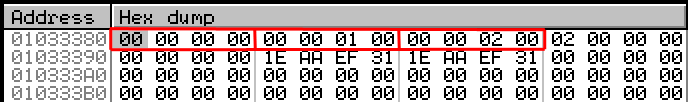
\includegraphics[width=0.6\textwidth]{patterns/13_arrays/5_multidimensional/olly_2D_2.png}
\caption{\olly: array is filled}
\end{figure}


\subsubsection{Access two-dimensional array as one-dimensional}

We can be easily assured that it's possible to access a two-dimensional array as one-dimensional array in at least two ways:

\lstinputlisting[style=customc]{patterns/13_arrays/5_multidimensional/2D_as_1D_EN.c}

Compile and run it: it shows correct values.

What MSVC 2013 did is fascinating, all three routines are just the same!

\lstinputlisting[caption=\Optimizing MSVC 2013 x64,style=customasmx86]{patterns/13_arrays/5_multidimensional/2D_as_1D_MSVC_2013_Ox_x64_EN.asm}

GCC also generates equivalent routines, but slightly different:

\lstinputlisting[caption=\Optimizing GCC 4.9 x64,style=customasmx86]{patterns/13_arrays/5_multidimensional/2D_as_1D_GCC49_x64_O3_EN.s}


\subsubsection{Three-dimensional array example}

It's the same for multidimensional arrays.

Now we are going to work with an array of type \Tint: each element requires 4 bytes in memory.

Let's see:

\lstinputlisting[caption=simple example,style=customc]{patterns/13_arrays/5_multidimensional/multi.c}

\myparagraph{x86}

We get (MSVC 2010):

\lstinputlisting[caption=MSVC 2010,style=customasmx86]{patterns/13_arrays/5_multidimensional/multi_msvc_EN.asm}

Nothing special. For index calculation, three input arguments are used 
in the formula $address=600 \cdot 4 \cdot x + 30 \cdot 4 \cdot y + 4z$, to represent the array as multidimensional.
Do not forget that the \Tint type is 32-bit (4 bytes),
so all coefficients must be multiplied by 4.

\lstinputlisting[caption=GCC 4.4.1,style=customasmx86]{patterns/13_arrays/5_multidimensional/multi_gcc_EN.asm}

The GCC compiler does it differently.

For one of the operations in the calculation ($30y$), GCC produces code without multiplication instructions.
This is how it done: 
$(y+y) \ll 4 - (y+y) = (2y) \ll 4 - 2y = 2 \cdot 16 \cdot y - 2y = 32y - 2y = 30y$. 
Thus, for the $30y$ calculation, only one addition operation,
one bitwise shift operation and one subtraction operation are used.
This works faster.

\myparagraph{ARM + \NonOptimizingXcodeIV (\ThumbMode)}

\lstinputlisting[caption=\NonOptimizingXcodeIV (\ThumbMode),style=customasmARM]{patterns/13_arrays/5_multidimensional/multi_Xcode_thumb_O0_EN.asm}

\NonOptimizing LLVM saves all variables in local stack, which is redundant.

The address of the array element is calculated by the formula we already saw.

\myparagraph{ARM + \OptimizingXcodeIV (\ThumbMode)}

\lstinputlisting[caption=\OptimizingXcodeIV (\ThumbMode),style=customasmARM]{patterns/13_arrays/5_multidimensional/multi_Xcode_thumb_O3_EN.asm}

The tricks for replacing multiplication by shift, addition and subtraction which we already saw
are also present here.

\myindex{ARM!\Instructions!RSB}
\myindex{ARM!\Instructions!SUB}
Here we also see a new instruction for us: \RSB (\IT{Reverse Subtract}).

It works just as \SUB, but it swaps its operands with each other before execution.
Why?
\myindex{ARM!Optional operators!LSL}
\SUB and \RSB  are instructions, to the second operand of which shift coefficient may be applied: (\INS{LSL\#4}). 

But this coefficient can be applied only to second operand.

That's fine for commutative operations like addition or multiplication 
(operands may be swapped there without changing the result).

But subtraction is a non-commutative operation, so \RSB exist for these cases.

\myparagraph{MIPS}

\myindex{MIPS!Global Pointer}
My example is tiny, so the GCC compiler decided to put the $a$ array into the 64KiB area 
addressable by the Global Pointer.

\lstinputlisting[caption=\Optimizing GCC 4.4.5 (IDA),style=customasmMIPS]{patterns/13_arrays/5_multidimensional/multi_MIPS_O3_IDA_EN.lst}



\subsubsection{More examples}

The computer screen is represented as a 2D array, but the video-buffer is a linear 1D array. 
We talk about it here: \myref{Mandelbrot_demo}.

Another example in this book is Minesweeper game: it's field is also two-dimensional array: \ref{minesweeper_winxp}.

}
\RU{\subsection{Многомерные массивы}

Внутри многомерный массив выглядит так же как и линейный.

Ведь память компьютера линейная, это одномерный массив.
Но для удобства этот одномерный массив легко представить как многомерный.

К примеру, вот как элементы массива 3x4 расположены в одномерном массиве из 12 ячеек:

% TODO FIXME not clear. First, horizontal would be better. Second, why two columns?
% I'd first show 3x4 with numbered elements (e.g. 32-bit ints) in colored lines,
% then linear with the same numbered elements (and colored blocks)
% then linear with addresses (offsets) - assuming let say 32-bit ints.
\begin{table}[H]
\centering
\begin{tabular}{ | l | l | }
\hline
Смещение в памяти & элемент массива \\
\hline
0 & [0][0] \\
\hline
1 & [0][1] \\
\hline
2 & [0][2] \\
\hline
3 & [0][3] \\
\hline
4 & [1][0] \\
\hline
5 & [1][1] \\
\hline
6 & [1][2] \\
\hline
7 & [1][3] \\
\hline
8 & [2][0] \\
\hline
9 & [2][1] \\
\hline
10 & [2][2] \\
\hline
11 & [2][3] \\
\hline
\end{tabular}
\caption{Двухмерный массив представляется в памяти как одномерный}
\end{table}

Вот по каким адресам в памяти располагается каждая ячейка двухмерного массива 3*4:

\begin{table}[H]
\centering
\begin{tabular}{ | l | l | l | l | }
\hline                        
0 & 1 & 2 & 3 \\
\hline  
4 & 5 & 6 & 7 \\
\hline  
8 & 9 & 10 & 11 \\
\hline  
\end{tabular}
\caption{Адреса в памяти каждой ячейки двухмерного массива}
\end{table}

\myindex{row-major order}
Чтобы вычислить адрес нужного элемента, сначала умножаем первый индекс (строку) на 4 (ширину массива), 
затем прибавляем второй индекс (столбец).

Это называется \IT{row-major order}, 
и такой способ представления массивов и матриц используется по крайней мере в \CCpp и Python. 
Термин \IT{row-major order} означает по-русски примерно следующее: \q{сначала записываем элементы первой строки, затем второй,~\dots~и~элементы последней 
строки в самом конце}.

\myindex{column-major order}
\myindex{Фортран}
Другой способ представления называется \IT{column-major order} (индексы массива используются в обратном порядке) 
и это используется по крайней мере в Фортране, MATLAB и R. 
Термин \IT{column-major order} означает по-русски
следующее: \q{сначала записываем элементы первого столбца, затем второго,~\dots~и~элементы последнего столбца
в самом конце}.

Какой из способов лучше?
В терминах производительности и кэш-памяти, лучший метод организации данных это тот,
при котором к данным обращаются последовательно.

Так что если ваша функция обращается к данным построчно, то \IT{row-major order} лучше,
и наоборот.

% subsections
\subsubsection{Пример с двумерным массивов}

Мы будем работать с массивом типа \Tchar. Это значит, что каждый элемент требует
только одного байта в памяти.

\myparagraph{Пример с заполнением строки}
\myindex{\olly}

Заполняем вторую строку значениями 0..3:

\lstinputlisting[caption=Пример с заполнением строки,style=customc]{patterns/13_arrays/5_multidimensional/two1_RU.c}

Все три строки обведены красным. 
Видно, что во второй теперь имеются байты 0, 1, 2 и 3:

\begin{figure}[H]
\centering
\includegraphics[width=0.6\textwidth]{patterns/13_arrays/5_multidimensional/olly_2D_1.png}
\caption{\olly: массив заполнен}
\end{figure}

\myparagraph{Пример с заполнением столбца}
\myindex{\olly}

Заполняем третий столбец значениями 0..2:

\lstinputlisting[caption=Пример с заполнением столбца,style=customc]{patterns/13_arrays/5_multidimensional/two2_RU.c}

Здесь также обведены красным три строки. 
Видно, что в каждой строке, на третьей позиции, теперь записаны 0, 1 и 2.

\begin{figure}[H]
\centering
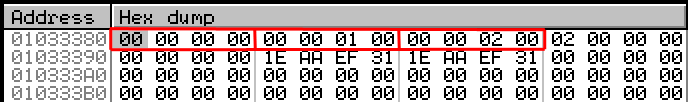
\includegraphics[width=0.6\textwidth]{patterns/13_arrays/5_multidimensional/olly_2D_2.png}
\caption{\olly: массив заполнен}
\end{figure}

\subsubsection{Работа с двухмерным массивом как с одномерным}

Мы можем легко убедиться, что можно работать с двухмерным массивом как с одномерным,
используя по крайней мере два метода:

\lstinputlisting[style=customc]{patterns/13_arrays/5_multidimensional/2D_as_1D_RU.c}

Компилируете и запускаете: мы увидим корректные значения.

Очарователен результат работы MSVC 2013~--- все три процедуры одинаковые!

\lstinputlisting[caption=\Optimizing MSVC 2013 x64,style=customasmx86]{patterns/13_arrays/5_multidimensional/2D_as_1D_MSVC_2013_Ox_x64_RU.asm}

GCC сгенерировал практически одинаковые процедуры:

\lstinputlisting[caption=\Optimizing GCC 4.9 x64,style=customasmx86]{patterns/13_arrays/5_multidimensional/2D_as_1D_GCC49_x64_O3_RU.s}


\subsubsection{Пример с трехмерным массивом}

То же самое и для многомерных массивов.
На этот раз будем работать с массивом типа \Tint: каждый элемент требует 4 байта в памяти.

Попробуем:

\lstinputlisting[caption=простой пример,style=customc]{patterns/13_arrays/5_multidimensional/multi.c}

\myparagraph{x86}

В итоге (MSVC 2010):

\lstinputlisting[caption=MSVC 2010,style=customasmx86]{patterns/13_arrays/5_multidimensional/multi_msvc_RU.asm}

В принципе, ничего удивительного. В \TT{insert()} для вычисления адреса нужного элемента массива 
три входных аргумента перемножаются по формуле $address=600 \cdot 4 \cdot x + 30 \cdot 4 \cdot y + 4z$, 
чтобы представить массив трехмерным.
Не забывайте также, что тип \Tint 32-битный (4 байта), поэтому все коэффициенты нужно умножить на 4.

\lstinputlisting[caption=GCC 4.4.1,style=customasmx86]{patterns/13_arrays/5_multidimensional/multi_gcc_RU.asm}

Компилятор GCC решил всё сделать немного иначе.
Для вычисления одной из операций ($30y$), GCC создал код, где нет самой операции умножения.

Происходит это так: 
$(y+y) \ll 4 - (y+y) = (2y) \ll 4 - 2y = 2 \cdot 16 \cdot y - 2y = 32y - 2y = 30y$. 
Таким образом, для вычисления $30y$ используется только операция сложения, 
операция битового сдвига и операция вычитания.
Это работает быстрее.

\myparagraph{ARM + \NonOptimizingXcodeIV (\ThumbMode)}

\lstinputlisting[caption=\NonOptimizingXcodeIV (\ThumbMode),style=customasmARM]{patterns/13_arrays/5_multidimensional/multi_Xcode_thumb_O0_RU.asm}

\NonOptimizing LLVM сохраняет все переменные в локальном стеке, хотя это и избыточно.

Адрес элемента массива вычисляется по уже рассмотренной формуле.

\myparagraph{ARM + \OptimizingXcodeIV (\ThumbMode)}

\lstinputlisting[caption=\OptimizingXcodeIV (\ThumbMode),style=customasmARM]{patterns/13_arrays/5_multidimensional/multi_Xcode_thumb_O3_RU.asm}

Тут используются уже описанные трюки для замены умножения на операции сдвига, сложения и вычитания.

\myindex{ARM!\Instructions!RSB}
\myindex{ARM!\Instructions!SUB}
Также мы видим новую для себя инструкцию \RSB (\IT{Reverse Subtract}).
Она работает так же, как и \SUB, только меняет операнды местами.

Зачем?
\myindex{ARM!Optional operators!LSL}
\SUB и \RSB это те инструкции, ко второму операнду которых можно применить коэффициент сдвига, как мы видим и здесь: (\INS{LSL\#4}). 
Но этот коэффициент можно применить только ко второму операнду.

Для коммутативных операций, таких как сложение или умножение, 
операнды можно менять местами и это не влияет на результат.

Но вычитание~--- операция некоммутативная, так что для этих случаев существует инструкция \RSB.

\myparagraph{MIPS}

\myindex{MIPS!Global Pointer}

Мой пример такой крошечный, что компилятор GCC решил разместить массив $a$ в 64KiB-области,
адресуемой при помощи Global Pointer.

\lstinputlisting[caption=\Optimizing GCC 4.4.5 (IDA),style=customasmMIPS]{patterns/13_arrays/5_multidimensional/multi_MIPS_O3_IDA_RU.lst}



\subsubsection{Ещё примеры}

Компьютерный экран представляет собой двумерный массив, но видеобуфер это линейный
одномерный массив. 
Мы рассматриваем это здесь: \myref{Mandelbrot_demo}.

Еще один пример в этой книге это игра ``Сапер'': её поле это тоже двухмерный массив: \ref{minesweeper_winxp}.

}
\DE{\subsection{Multidimensionale Arrays}
Intern ist ein multidimensionales Array im Prinzip das gleiche wie ein lineares Array.

Da der Speicher eines Rechners linear ist, ist es ein eindimensionales Array.
Zur Vereinfachung kann dieses multidimensionales Array leicht als eindimensional dargestellt werden.

Beispielsweise werden die Elemente eines 3x4 Arrays folgendermaßen in einem eindimensionalen Array aus 12 Zellen
gespeichert:

% TODO FIXME not clear. First, horizontal would be better. Second, why two columns?
% I'd first show 3x4 with numbered elements (e.g. 32-bit ints) in colored lines,
% then linear with the same numbered elements (and colored blocks)
% then linear with addresses (offsets) - assuming let say 32-bit ints.
\begin{table}[H]
\centering
\begin{tabular}{ | l | l | }
\hline
Offset im Speicher & Arrayelement \\
\hline
0 & [0][0] \\
\hline
1 & [0][1] \\
\hline
2 & [0][2] \\
\hline
3 & [0][3] \\
\hline
4 & [1][0] \\
\hline
5 & [1][1] \\
\hline
6 & [1][2] \\
\hline
7 & [1][3] \\
\hline
8 & [2][0] \\
\hline
9 & [2][1] \\
\hline
10 & [2][2] \\
\hline
11 & [2][3] \\
\hline
\end{tabular}
\caption{Zweidimensionales Array in eindimensionaler Speicherdarstellung}
\end{table}

Auf diese Weise wird jede Zellen des 3*4 Arrays im Speicher abgelegt:

% TODO coordinates. TikZ?
\begin{table}[H]
\centering
\begin{tabular}{ | l | l | l | l | }
\hline                        
0 & 1 & 2 & 3 \\
\hline  
4 & 5 & 6 & 7 \\
\hline  
8 & 9 & 10 & 11 \\
\hline  
\end{tabular}
\caption{Speicheradressen jeder Zelle des zweidimensionalen Arrays}
\end{table}

\myindex{row-major order}
Um also die Adresse des benötigten Elements zu berechnen, multiplizieren wir zunächst den ersten Index mit 4 (der
Arraybreite) und addieren dann den zweiten Index.
Dies nennt man \IT{Zeilenordnung} (engl. row-major order) und diese Methode zur Darstellung von Arrays und Matrizen
wird mindestens von \CCpp und Python verwendet.
Der Ausdruck row-major order bedeutet: \q{schreibe zuerst die Elemente der ersten Zeilen, dann die zweite Zeile\dots
und schließlich die Elemente der letzten Zeile}.

\myindex{column-major order}
\myindex{Fortran}
Eine andere Methode zur Darstellung heißt \IT{Spaltenordnung} (engl. column-major order) (die Indizes des Arrays werden
in umgekehrter Reihenfolge verwendet) und wird zumindest in Fortran, MATLAB und R verwendet.
Der Ausdruck column-major oder bedeutet: \q{schreibe zuerst die Elemente der ersten Spalte, dann die zweite Spalte\dots
und schließlich die Elemente der letzten Spalte}.

Welche Method ist besser?

Generel ist hinsichtlich Performance und Cachespeicher die beste Methode der Datenorganisation diejenige, in der auf die
Elemente sequentiell zugegriffen wird.

Wenn eine Funktion auf Daten zeilenweise zugreift, ist Zeilenordnung besser und umgekehrt.

% subsections
\subsubsection{Beispiel für zweidimensionales Array}
Wir werden mit einem Array vom Typ \Tchar arbeiten, was bedeutet, dass jedes Element nur ein Byte Speicherplatz
benötigt.


\myparagraph{Beispiel: Zeile füllen}
\myindex{\olly}
Füllen wir die zweite Zeilen mit den Werten 0..3:

\lstinputlisting[caption=Row filling example,style=customc]{patterns/13_arrays/5_multidimensional/two1_DE.c}
Alle drei Zeilen sind rot markiert.
Wir erkennen, dass die zweite Zeilen nun die Werte 0,1,2 und 3 enthält:

\begin{figure}[H]
\centering
\includegraphics[width=0.6\textwidth]{patterns/13_arrays/5_multidimensional/olly_2D_1.png}
\caption{\olly: Array ist befüllt}
\end{figure}

\myparagraph{Beipsiel: Spalte füllen}
\myindex{\olly}
Füllen wir die dritte Spalte mit den Werten 0..2:

\lstinputlisting[caption=Column filling example,style=customc]{patterns/13_arrays/5_multidimensional/two2_DE.c}

Die drei Spalten sind hier ebenfalls rot markiert.

Wir erkennen, dass sich in jeder Zeile an der dritten Stelle die Werte 0,1 und 2 befinden. 

\begin{figure}[H]
\centering
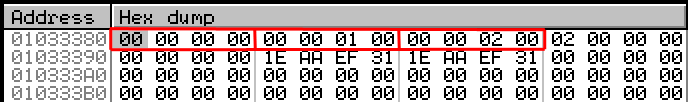
\includegraphics[width=0.6\textwidth]{patterns/13_arrays/5_multidimensional/olly_2D_2.png}
\caption{\olly: Array ist befüllt}
\end{figure}


\subsubsection{Eindimensionaler Zugriff auf zweidimensionales Array}
Wir können uns leicht davon überzeugen, dass es auf mindestens zwei Arten möglich ist, auf ein zweidimensionales Array
eindimensional zuzugreifen:

\lstinputlisting[style=customc]{patterns/13_arrays/5_multidimensional/2D_as_1D_DE.c}

Kompilieren und ausführen: es zeigt korrekte Werte an
Was MSVC 2013 getan hat ist faszinierend: alle drei Routinen sind identisch!

\lstinputlisting[caption=\Optimizing MSVC 2013 x64,style=customasmx86]{patterns/13_arrays/5_multidimensional/2D_as_1D_MSVC_2013_Ox_x64_EN.asm}

GCC erzeugt ebenfalls äquivalente Routinen, aber ein wenig anders:

\lstinputlisting[caption=\Optimizing GCC 4.9 x64,style=customasmx86]{patterns/13_arrays/5_multidimensional/2D_as_1D_GCC49_x64_O3_EN.s}


\subsubsection{Beispiel: dreidimensionales Array}

Mit multidimensionalen Arrays ist es das gleiche.

Wir werden nun mit einem Array vom Typ \Tint arbeiten: jedes Element benötigt 4 Byte Speicherplatz.

Sehen wir es uns an:

\lstinputlisting[caption=simple example,style=customc]{patterns/13_arrays/5_multidimensional/multi.c}

\myparagraph{x86}

Wir erhalten das Folgende (MSVC 2010):

\lstinputlisting[caption=MSVC 2010,style=customasmx86]{patterns/13_arrays/5_multidimensional/multi_msvc_DE.asm}
Nichts Außergewöhnliches. Zur Berechnung des Index' werden in der Formel $address=600 \cdot 4 \cdot x + 30 \cdot 4 \cdot
y + 4z$ drei Eingabewerte verwendet, um das multidimensionale Array zu repräsentieren.
Vergessen wir nicht, dass der \Tint Typ 32 Bit (4 Byte) breit ist, sodass alle Koeffizienten mit 4 multipliziert werden
müssen.

\lstinputlisting[caption=GCC 4.4.1,style=customasmx86]{patterns/13_arrays/5_multidimensional/multi_gcc_DE.asm}
Der GCC Compiler arbeitet anders.

Für eine der Operationen in der Berechnung ($30y$) produziet GCC Code ohne Multiplikationsbefehle.
Das funktioniert wie folgt:
$(y+y) \ll 4 - (y+y) = (2y) \ll 4 - 2y = 2 \cdot 16 \cdot y - 2y = 32y - 2y = 30y$.

So werden für die $30y$ Berechnung nur ein Addierbefehl, eine bitweiser Verschiebebefehl und ein Subtraktionsbefehl
verwendet. So geht es schneller.

\myparagraph{ARM + \NonOptimizingXcodeIV (\ThumbMode)}

\lstinputlisting[caption=\NonOptimizingXcodeIV
(\ThumbMode),style=customasmARM]{patterns/13_arrays/5_multidimensional/multi_Xcode_thumb_O0_DE.asm}

\NonOptimizing LLVM speichert alle Variablen auf dem lokalen Stack, was redundant ist.

Die Adresse des Arrayelements wird über die eben gezeigte Formel berechnet.

\myparagraph{ARM + \OptimizingXcodeIV (\ThumbMode)}

\lstinputlisting[caption=\OptimizingXcodeIV
(\ThumbMode),style=customasmARM]{patterns/13_arrays/5_multidimensional/multi_Xcode_thumb_O3_DE.asm}
Die Tricks für das Ersetzen der Multiplikation durch Verschieben, Addieren und Subtrahieren, die wir bereits
kennengelernt haben, kommen hier auch vor.

\myindex{ARM!\Instructions!RSB}
\myindex{ARM!\Instructions!SUB}
Hier finden wir auch einen für uns neuen Befehl: \RSB (\IT{Reverse Subtract}).

Er arbeitet genau wie \SUB, aber vertauscht die Operanden vor der Ausführung. Warum?

\myindex{ARM!Optional operators!LSL}
\SUB und \RSB  sind Befehle, bei denen auf den zweiten Operanden eine bitweise Verschiebung angewendet werden kann:
(\INS{LSL\#4}).
Dieser Koeffizient kann aber nur auf den zweiten Operanden angewendet werden.

Das ist günstig für kommutative Operationen wie Addition und Multiplikation (die Operanden können vertauscht werden,
ohne das Ergebnis zu verändern).

Subtraktion dagegen ist nicht kommutativ, weshalb für diese Fälle \RSB existiert.

\myparagraph{MIPS}

\myindex{MIPS!Global Pointer}
Das Beispiel ist sehr klein, sodass der GCC Compiler entschieden hat das Array $a$ im 64KiB Platz abzulegen, um es durch
den globalen Pointer zugreifbar zu machen.

\lstinputlisting[caption=\Optimizing GCC 4.4.5
(IDA),style=customasmMIPS]{patterns/13_arrays/5_multidimensional/multi_MIPS_O3_IDA_DE.lst}



\subsubsection{Weitere Beispiele}
Der Bildschirm wird als 2D-Array dargestellt, aber der Videopuffer ist ein lineares 1D-Array.
Wir betrachten hier näher: \myref{Mandelbrot_demo}.

Ein anderes Beispiel in diesem Buch ist das Spiel Minesweeper: das Feld ist auch ein zweidimensionales Array:
\ref{minesweeper_winxp}.

}

\EN{\subsection{Pack of strings as a two-dimensional array}

Let's revisit the function that returns the name of a month: \lstref{get_month1}.

As you see, at least one memory load operation is needed to prepare a pointer to the string
that's the month's name.

Is it possible to get rid of this memory load operation?

In fact yes, if you represent the list of strings as a two-dimensional array:

\lstinputlisting[style=customc]{patterns/13_arrays/55_month_2D/month2_EN.c}

Here is what we've get:

\lstinputlisting[caption=\Optimizing MSVC 2013 x64,style=customasmx86]{patterns/13_arrays/55_month_2D/MSVC2013_x64_Ox_EN.asm}

There are no memory accesses at all.

All this function does is to calculate a point at which the first character of the name of the month is: 
$pointer\_to\_the\_table + month * 10$.

There are also two \LEA instructions, which effectively work as several \MUL and \MOV instructions.

The width of the array is 10 bytes. 

Indeed, the longest string here---\q{September}---is 9 bytes, and plus the terminating zero is 10 bytes.

The rest of the month names are padded by zero bytes, so they all occupy the same space (10 bytes).

Thus, our function works even faster, because all string start at an address which can be
calculated easily.

\Optimizing GCC 4.9 can do it even shorter:

\begin{lstlisting}[caption=\Optimizing GCC 4.9 x64,style=customasmx86]
	movsx	rdi, edi
	lea	rax, [rdi+rdi*4]
	lea	rax, month2[rax+rax]
	ret
\end{lstlisting}

\LEA is also used here for multiplication by 10.

Non-optimizing compilers do multiplication differently.

\lstinputlisting[caption=\NonOptimizing GCC 4.9 x64,style=customasmx86]{patterns/13_arrays/55_month_2D/x64_GCC49_O0_EN.asm}

\NonOptimizing MSVC just uses \IMUL instruction:
\myindex{x86!\Instructions!IMUL}

\lstinputlisting[caption=\NonOptimizing MSVC 2013 x64,style=customasmx86]{patterns/13_arrays/55_month_2D/MSVC2013_x64_EN.asm}

\myindex{\CompilerAnomaly}
\label{MSVC2013_anomaly}

But one thing is weird here: why add multiplication by zero and adding zero to the final result?

This looks like a compiler code generator quirk, which wasn't caught by the compiler's tests
(the resulting code works correctly, after all).
% класс!
%
We intentionally consider such pieces of code so the reader would understand, 
that sometimes one shouldn't puzzle over such compiler artifacts.

\subsubsection{32-bit ARM}

\Optimizing Keil 
for Thumb mode uses the multiplication instruction \INS{MULS}:

\lstinputlisting[caption=\OptimizingKeilVI (\ThumbMode),style=customasmARM]{patterns/13_arrays/55_month_2D/Keil_O3_thumb_EN.asm}

\Optimizing Keil for ARM mode uses add and shift operations:

\lstinputlisting[caption=\OptimizingKeilVI (\ARMMode),style=customasmARM]{patterns/13_arrays/55_month_2D/Keil_O3_ARM_EN.asm}

\subsubsection{ARM64}

\lstinputlisting[caption=\Optimizing GCC 4.9 ARM64,style=customasmARM]{patterns/13_arrays/55_month_2D/GCC49_ARM64_EN.asm}

\myindex{ARM!\Instructions!SXTW}
\myindex{ARM!\Instructions!ADRP/ADD pair}

\INS{SXTW} is used for sign-extension and promoting input 32-bit value into a 64-bit one and storing it in X0.

\ADRP/\ADD pair is used for loading the address of the table.

The \ADD instructions also has a \LSL suffix, which helps with multiplications.

\subsubsection{MIPS}
\lstinputlisting[caption=\Optimizing GCC 4.4.5 (IDA),style=customasmMIPS]{patterns/13_arrays/55_month_2D/MIPS_O3_IDA_EN.lst}

\subsubsection{\Conclusion{}}

This is a bit old-school technique to store text strings.
You may find a lot of it in \oracle, for example.
It's hard to say if it's worth doing on modern computers.
Nevertheless, it is a good example of arrays, so it was added to this book.

}
\RU{\subsection{Набор строк как двухмерный массив}

Снова вернемся к примеру, который возвращает название месяца: \lstref{get_month1}.
Как видно, нужна как минимум одна операция загрузки из памяти для подготовки указателя на строку,
состоящую из имени месяца.

Возможно ли избавиться от операции загрузки из памяти?

Да, если представить список строк как двумерный массив:

\lstinputlisting[style=customc]{patterns/13_arrays/55_month_2D/month2_RU.c}

Вот что получаем:

\lstinputlisting[caption=\Optimizing MSVC 2013 x64,style=customasmx86]{patterns/13_arrays/55_month_2D/MSVC2013_x64_Ox_RU.asm}

Здесь нет обращений к памяти вообще.
Эта функция только вычисляет место, где находится первый символ названия месяца:
 
$pointer\_to\_the\_table + month * 10$.
Там также две инструкции \LEA, которые работают как несколько инструкций \MUL и \MOV.

Ширина массива~--- 10 байт. 
Действительно, самая длинная строка это \q{September} (9 байт) плюс оконечивающий ноль, получается 10 байт.

Остальные названия месяцев дополнены нулевыми байтами, чтобы они занимали столько же места (10 байт).

Таким образом, наша функция и работает быстрее, потому что все строки начинаются с тех адресов, 
которые легко вычислить.

\Optimizing GCC 4.9 может ещё короче:

\begin{lstlisting}[caption=\Optimizing GCC 4.9 x64,style=customasmx86]
	movsx	rdi, edi
	lea	rax, [rdi+rdi*4]
	lea	rax, month2[rax+rax]
	ret
\end{lstlisting}

\LEA здесь также используется для умножения на 10.

Неоптимизирующие компиляторы делают умножение по-разному.

\lstinputlisting[caption=\NonOptimizing GCC 4.9 x64,style=customasmx86]{patterns/13_arrays/55_month_2D/x64_GCC49_O0_RU.asm}

\NonOptimizing MSVC просто использует инструкцию \IMUL:
\myindex{x86!\Instructions!IMUL}

\lstinputlisting[caption=\NonOptimizing MSVC 2013 x64,style=customasmx86]{patterns/13_arrays/55_month_2D/MSVC2013_x64_RU.asm}

\myindex{\CompilerAnomaly}
\label{MSVC2013_anomaly}
Но вот что странно: зачем добавлять умножение на ноль и добавлять ноль к конечному результату?

Это выглядит как странность кодегенератора компилятора, который не был покрыт тестами
компилятора. Но так или иначе, итоговый код работает корректно.
% класс! ЩИТО?
Мы сознательно рассматриваем такие фрагменты кода, чтобы читатель понимал, что иногда не нужно
ломать себе голову над подобными артефактами компиляторов.

\subsubsection{32-bit ARM}

\Optimizing Keil для режима Thumb использует инструкцию умножения \INS{MULS}:

\lstinputlisting[caption=\OptimizingKeilVI (\ThumbMode),style=customasmARM]{patterns/13_arrays/55_month_2D/Keil_O3_thumb_RU.asm}

\Optimizing Keil для режима ARM использует операции сложения и сдвига:

\lstinputlisting[caption=\OptimizingKeilVI (\ARMMode),style=customasmARM]{patterns/13_arrays/55_month_2D/Keil_O3_ARM_RU.asm}

\subsubsection{ARM64}

\lstinputlisting[caption=\Optimizing GCC 4.9 ARM64,style=customasmARM]{patterns/13_arrays/55_month_2D/GCC49_ARM64_RU.asm}

\myindex{ARM!\Instructions!SXTW}
\myindex{ARM!\Instructions!ADRP/ADD pair}
\INS{SXTW} используется для знакового расширения и расширения
входного 32-битного значения в 64-битное и сохранения его в X0.

Пара \ADRP/\ADD используется для загрузки адреса таблицы.

У инструкции \ADD также есть суффикс \LSL, что помогает с умножением.

\subsubsection{MIPS}
\lstinputlisting[caption=\Optimizing GCC 4.4.5 (IDA),style=customasmMIPS]{patterns/13_arrays/55_month_2D/MIPS_O3_IDA_RU.lst}

\subsubsection{\Conclusion{}}

Это немного олд-скульная техника для хранения текстовых строк.
Много такого можно найти в \oracle, например.
Трудно сказать, стоит ли оно того на современных компьютерах.
Так или иначе, это был хороший пример массивов, поэтому он был добавлен в эту книгу.

}
\DE{\subsection{Strings als zweidimensionales Array}
Betrachten wir erneut die Funktion, die den Namen eines Monats zurückgibt: \lstref{get_month1}.

Wie man sieht wird mindestens eine Befehl benötigt, der einen Wert aus dem Speicher lädt, um den Pointer auf den String,
der den Monatsnamen enthält, vorzubereiten.

Ist es möglich diesen Speicherzugriff loszuwerden?

Die Antwort ist: ja, wenn man die Liste aus String als zweidimensionales Array darstellt:

\lstinputlisting[style=customc]{patterns/13_arrays/55_month_2D/month2_DE.c}

Hier ist was wir erhalten:

\lstinputlisting[caption=\Optimizing MSVC 2013
x64,style=customasmx86]{patterns/13_arrays/55_month_2D/MSVC2013_x64_Ox_DE.asm}

Es gibt überhaupt keine Speicherzugriffe.
Alles, was diese Funktion tut, ist einen Pointer zu berechnen, der auf den ersten Buchstaben des Monats
zeigt:$pointer\_to\_the\_table + month \cdot 10$.

Es gibt auch zwei \LEA Befehle, die wie mehrere \MUL und \MOV Befehle funktionieren.

Die Breite des Arrays beträgt 10 Byte.

Der längste String im Beispiel---\q{September}---hat eine Länge von 9 Byte zuzüglich einer terminierenden Null, also
insgesamt 10 Byte.

Die übrigen Monatsnamen werden mit Zerobytes aufgefüllt, sodass alle denselben Speicherplatz (10 Byte) benötigen.

Dadurch arbeitet unsere Funktion noch schneller, denn die Startadresse jedes Strings kann so einfach berechnet werden.

\Optimizing GCC 4.9 kann sogar noch kürzeren Code erzeugen:

\begin{lstlisting}[caption=\Optimizing GCC 4.9 x64,style=customasmx86]
	movsx	rdi, edi
	lea	rax, [rdi+rdi*4]
	lea	rax, month2[rax+rax]
	ret
\end{lstlisting}

\LEA wird hier auch für die Multiplikation mit 10 verwendet.

Nicht optimierende Compiler führen die Multiplikation anders durch.

\lstinputlisting[caption=\NonOptimizing GCC 4.9
x64,style=customasmx86]{patterns/13_arrays/55_month_2D/x64_GCC49_O0_DE.asm}

\NonOptimizing MSVC verwendet nur den \IMUL Befehl:
\myindex{x86!\Instructions!IMUL}

\lstinputlisting[caption=\NonOptimizing MSVC 2013
x64,style=customasmx86]{patterns/13_arrays/55_month_2D/MSVC2013_x64_DE.asm}

\myindex{\CompilerAnomaly}
\label{MSVC2013_anomaly}
Eine Sache hier ist seltsam: warum wird die Multiplikation mit null und die Addition von null zum Endergebnis
hinzugefügt?

Dies sieht wie ein Fehler im Codegenerator des Compilers aus, der nicht durch die Tests des Compilers abgefangen wurde.
(Trotzdem funktioniert der erzeugte Code korrekt.)

% класс!
%
Wir betrachten solche Codes ganz bewußt, damit der Leser sich klarmacht, dass man sich über solche Merkwürdigkeiten und
Artefakte des Compilers nicht allzu sehr wundern soll.

\subsubsection{32-bit ARM}

\Optimizing Keil im Thumb mode verwendet zur Multiplikation den Befehl \INS{MULS}:

\lstinputlisting[caption=\OptimizingKeilVI
(\ThumbMode),style=customasmARM]{patterns/13_arrays/55_month_2D/Keil_O3_thumb_DE.asm}

\Optimizing Keil für ARM mode verwendet Additions- und Schiebebefehle:

\lstinputlisting[caption=\OptimizingKeilVI
(\ARMMode),style=customasmARM]{patterns/13_arrays/55_month_2D/Keil_O3_ARM_DE.asm}

\subsubsection{ARM64}

\lstinputlisting[caption=\Optimizing GCC 4.9
ARM64,style=customasmARM]{patterns/13_arrays/55_month_2D/GCC49_ARM64_DE.asm}

\myindex{ARM!\Instructions!SXTW}
\myindex{ARM!\Instructions!ADRP/ADD pair}
\INS{SXTW} wird für Vorzeichenerweiterung und Übertragung von 32-Bit-Werten in 64-Bit-Werte und das Speichern in X0
verwendet.

Das \ADRP/\ADD Paar wird für das Laden der Adresse der Tabelle verwendet.

Der \ADD Befehl trägt auch den \LSL Suffix, der bei der Multiplikation hilft.

\subsubsection{MIPS}
\lstinputlisting[caption=\Optimizing GCC 4.4.5 (IDA),style=customasmMIPS]{patterns/13_arrays/55_month_2D/MIPS_O3_IDA_EN.lst}

\subsubsection{\Conclusion{}}
Das Gezeigte ist eine etwas altmodische Technik um Textstrings zu speichern.
Man findet diesen Ansatz beispielsweise oft in \oracle.
Es ist schwer zu sagen, ob es sich für moderne Computer lohnt.
Nichtsdestotrotz ist es ein gutes Beispiel für Arrays und hat daher seine Berechtigung in diesem Buch.

}

\EN{\subsection{\Conclusion{}}

An array is a pack of values in memory located adjacently.

It's true for any element type, including structures.

Access to a specific array element is just a calculation of its address.
}
\RU{\subsection{\Conclusion{}}

Массив это просто набор значений в памяти, расположенных рядом друг с другом.

Это справедливо для любых типов элементов, включая структуры.

Доступ к определенному элементу массива это просто вычисление его адреса.

}
\DE{\subsection{\Conclusion{}}

Ein Array ist eine Ansammlung von Werten, die im Speicher nebeneinander angeordnet sind.

Dies gilt für alle Elementtypen und sogar für Structs.

Der Zugriff auf ein spezielles Element des Arrays entspricht lediglich eine Berechnung von dessen Adresse.}

\myindex{Hex-Rays}

\RU{\section{Кстати}
Итак, указатель на массив и адрес первого элемента --- это одно и то же.
Вот почему выражения \TT{ptr[0]} и \TT{*ptr} в \CCpp равноценны.
Любопытно что Hex-Rays часто заменяет первое вторым.
Он делает это в тех случаях, когда не знает, что имеет дело с указателем на целый массив,
и думает, что это указатель только на одну переменную.}%
\EN{\section{By the way}
So, pointer to an array and address of a first element---is the same thing.
This is why \TT{ptr[0]} and \TT{*ptr} expressions are equivalent in \CCpp.
It's interesting to note that Hex-Rays often replaces the first by the second.
It does so when it have no idea that it works with pointer to the whole array,
and thinks that this is a pointer to single variable.}
\DEph{}

\subsection{\Exercises}

\begin{itemize}
	\item \url{http://challenges.re/62}
	\item \url{http://challenges.re/63}
	\item \url{http://challenges.re/64}
	\item \url{http://challenges.re/65}
	\item \url{http://challenges.re/66}
\end{itemize}


